%%%%%%%%%%%%%%%%%%%%%%% file template.tex %%%%%%%%%%%%%%%%%%%%%%%%%
%
% This is a general template file for the LaTeX package SVJour3
% for Springer journals.          Springer Heidelberg 2010/09/16
%
% Copy it to a new file with a new name and use it as the basis
% for your article. Delete % signs as needed.
%
% This template includes a few options for different layouts and
% content for various journals. Please consult a previous issue of
% your journal as needed.
%
%%%%%%%%%%%%%%%%%%%%%%%%%%%%%%%%%%%%%%%%%%%%%%%%%%%%%%%%%%%%%%%%%%%
%
% First comes an example EPS file -- just ignore it and
% proceed on the \documentclass line
% your LaTeX will extract the file if required
\begin{filecontents*}{example.eps}
%!PS-Adobe-3.0 EPSF-3.0
%%BoundingBox: 19 19 221 221
%%CreationDate: Mon Sep 29 1997
%%Creator: programmed by hand (JK)
%%EndComments
gsave
newpath
  20 20 moveto
  20 220 lineto
  220 220 lineto
  220 20 lineto
closepath
2 setlinewidth
gsave
  .4 setgray fill
grestore
stroke
grestore
\end{filecontents*}
%
\RequirePackage{fix-cm}
%
%\documentclass{svjour3}                     % onecolumn (standard format)
%\documentclass[smallcondensed]{svjour3}     % onecolumn (ditto)
%\documentclass[smallextended]{svjour3}       % onecolumn (second format)
\documentclass[twocolumn]{svjour3}          % twocolumn
%
\smartqed  % flush right qed marks, e.g. at end of proof
%
\usepackage{bm}
\usepackage{graphicx}
\usepackage{epstopdf}
\usepackage{color}
\usepackage{multirow}
\usepackage{tabularx}
\usepackage[misc,geometry]{ifsym}
\usepackage{threeparttable}


\newcommand\todo[1]{\textcolor{red}{#1}}

%\usepackage{paralist}
%
% \usepackage{mathptmx}      % use Times fonts if available on your TeX system
%
% insert here the call for the packages your document requires
%\usepackage{latexsym}
% etc.
%
% please place your own definitions here and don't use \def but
% \newcommand{}{}
%
% Insert the name of "your journal" with
% \journalname{myjournal}
%
\begin{document}\sloppy


\title{Multi-modality Imagery Database for Plant Phenotyping \thanks{$^\star$ denotes equal contribution by the authors. This research was supported by Chemical Sciences, Geosciences and Biosciences Division, Office of Basic Energy Sciences, Office of Science, U.S. Department of Energy (award number DE-FG02-91ER20021), and by Center for Advanced Algal and Plant Phenotyping (CAAPP), Michigan State University.
}
}
%\subtitle{Do you have a subtitle?\\ If so, write it here}

%\titlerunning{Short form of title}        % if too long for running head

\author{Jeffrey A Cruz$^\star$ \and Xi Yin\footnote{Equal contributor}  \and Xiaoming Liu \and Saif M Imran \and Daniel~D~Morris \and David M Kramer    \and Jin Chen}

\authorrunning{Cruz {\it et al}} % if too long for running head

\institute{Jeffrey A Cruz $\cdot$ Jin Chen $\cdot$ David M Kramer \at
              Department of Energy Plant Research Laboratory, Michigan State University, East Lansing, MI 48824, USA  \\
		E-mail: \{cruzj,jinchen,kramerd8\}@msu.edu		
%             \emph{Present address:} of F. Author  %  if needed
           \and
           Xi Yin $\cdot$ Xiaoming Liu (\Letter)\at
              Department of Computer Science and Engineering, Michigan State University,  East Lansing, MI 48824, USA  \\
		E-mail: \{yinxi1,liuxm\}@cse.msu.edu
                      %  \\
              \and
           Saif Imran $\cdot$ Daniel D Morris \at
              Department of Electrical and Computer Engineering, Michigan State University,
              East Lansing, MI 48824, USA\\
		E-mail: \{imransai,dmorris\}@msu.edu
}

\date{Received: date / Accepted: date}
% The correct dates will be entered by the editor


\maketitle

\begin{abstract}

Among many applications of machine vision, plant image analysis has recently began to gain attention due to its potential impact on plant visual phenotyping, particularly in understanding plant growth, assessing the quality/performance of crop plants and improving crop yield. 
Despite its importance, the lack of publicly available research databases containing plant imagery has substantially hindered the advancement of plant image analysis. 
To alleviate this issue, this paper presents a new multi-modality plant imagery database named ``MSU-PID'', with two distinct properties. 
First, MSU-PID is captured using four types of imaging sensors, fluorescence, infrared (IR), RGB color, and depth. 
Second, the imaging setup and the variety of manual labels allow MSU-PID to be suitable for a diverse set of plant image analysis applications, such as leaf segmentation, leaf counting, leaf alignment, and leaf tracking. 
We provide detailed information on the plants, imaging sensors, calibration, labeling, and baseline performances of this new database.
%
%Among many applications of machine vision, plant image analysis has recently begin to gain attentions due to its potential huge impact to plant visual phenotyping, the understanding of plant growth, the quality of crops, and the improvement of the yield.
%Despite its importance, the pack of publicly available research database of plant imagery has substantially hindered the advancement of plant image analysis.
%To alleviate this issue, this paper presents a new multi-modality plant imagery database named ``MSU-PID'', with two distinct properties.
%First, MSU-PID is captured using four types of imaging sensors, Fluorescence, infrared (IR), RGB color, and depth.
%Second, the imaging setup and the variety of manual labels allow MSU-PID to be suitable for a diverse set of plant image analysis applications, such as leaf segmentation, leaf counting, leaf alignment, and leaf tracking.
%We provide detailed information on the plants, imaging sensors, calibration, labeling, and baseline performances of this new database.

\keywords{Plant Phenotyping  \and Computer Vision \and Plant image \and Leaf segmentation \and Leaf tracking\and Multiple sensors \and Arabidopsis \and Bean}
% \PACS{PACS code1 \and PACS code2 \and more}
% \subclass{MSC code1 \and MSC code2 \and more}
\end{abstract}

\section{Introduction}
\label{sec:intro}

With the rapid growth of world population and the loss of arable land, there is an increasing desire to improve the yield and quality of crops.  Key to increasing yields is gaining understanding of the genetic mechanisms that influence plant growth~\cite{doos2002population}.
%
A classic genetic approach is to produce a diverse population of mutant lines, grow them either in growth chambers with simulated environmental conditions or directly in the field, visually observe the plants during the growth period, and finally identify plant morphological or physiological patterns that tightly associate with key growth factors~\cite{houle2010phenomics}.
%
While many factors can be assessed quantitatively, which is essential for high-throughput study, one of the bottleneck in this research pipeline is plant visual phenotyping~\cite{walter2015plant}.

\begin{figure*}
\begin{centering}
\begin{tabular}{@{}c c c c c}
%\begin{tabular}{lllllllll}
(a) &
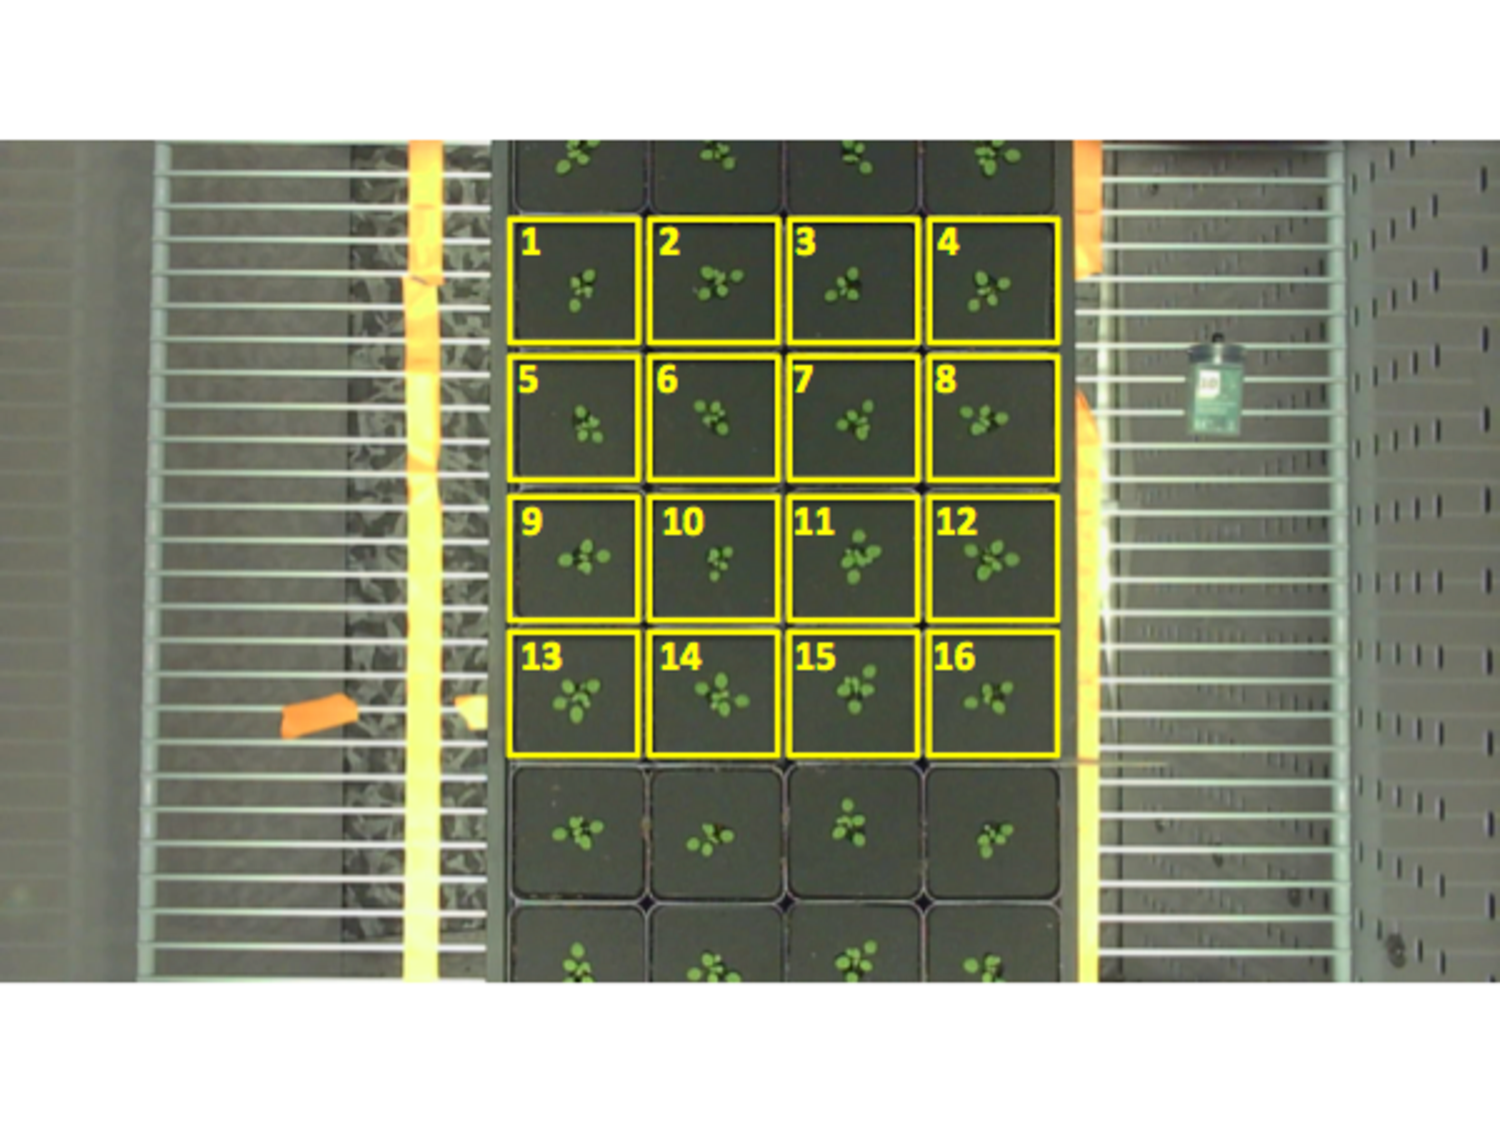
\includegraphics[width=.23\textwidth]{Figures/FourModalities/A_rgb}&
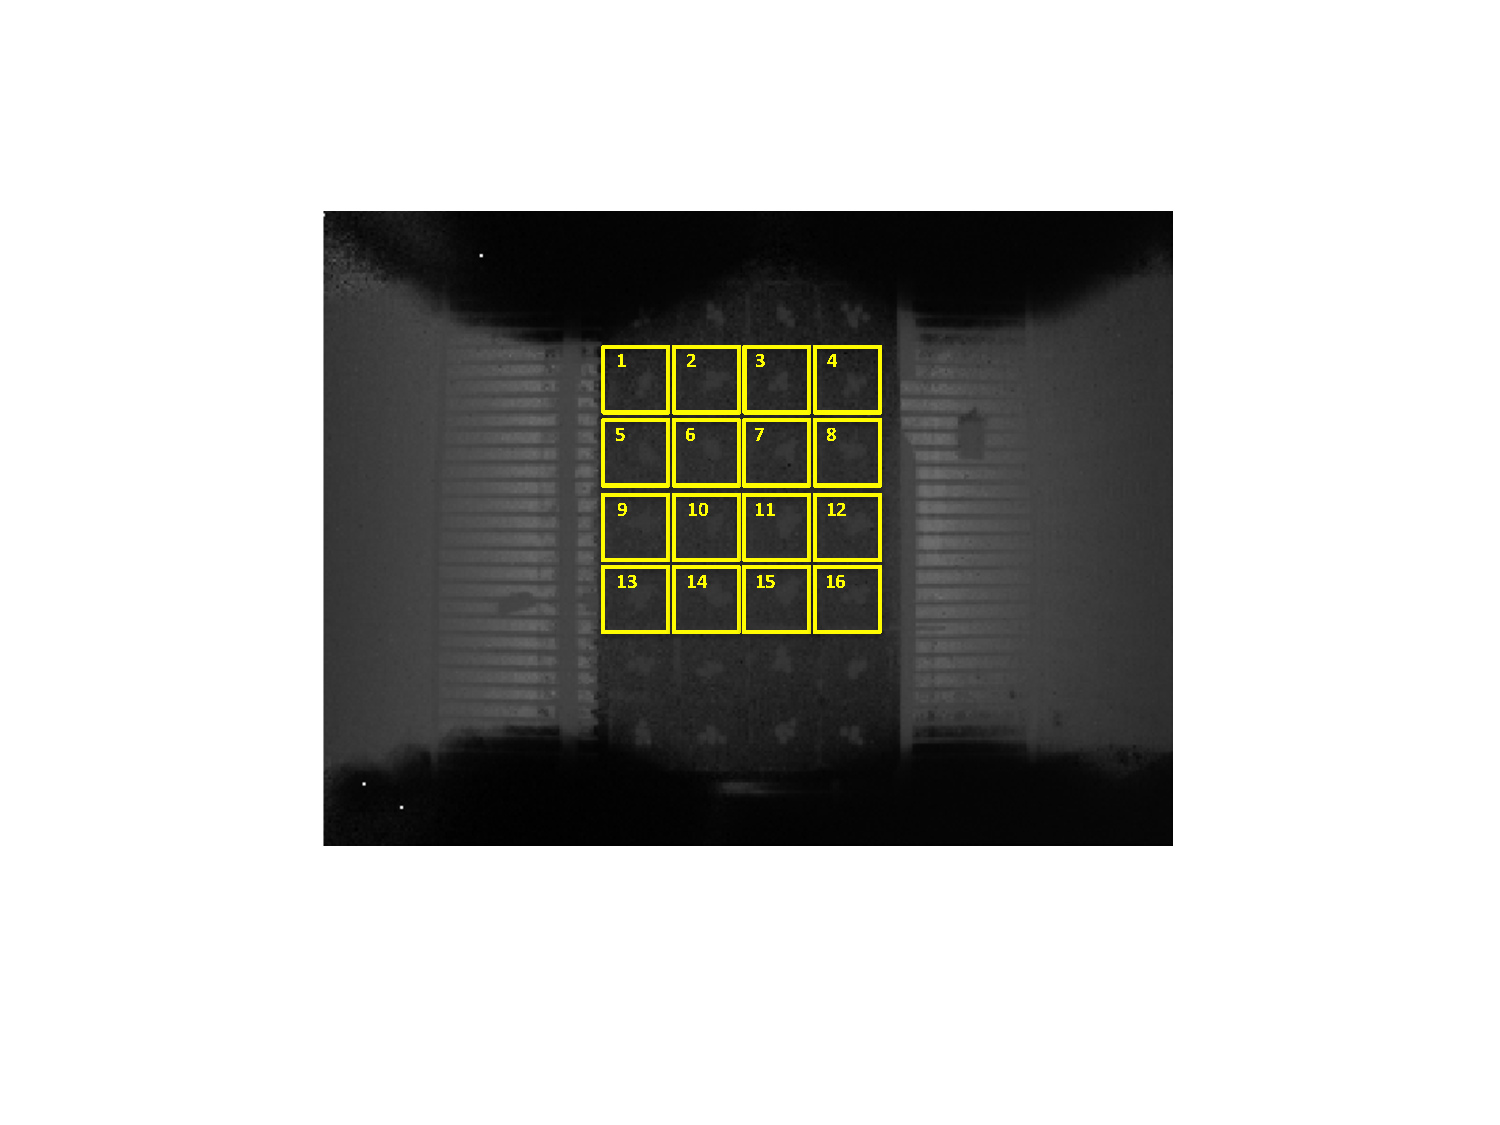
\includegraphics[width=.23\textwidth]{Figures/FourModalities/A_depth}&
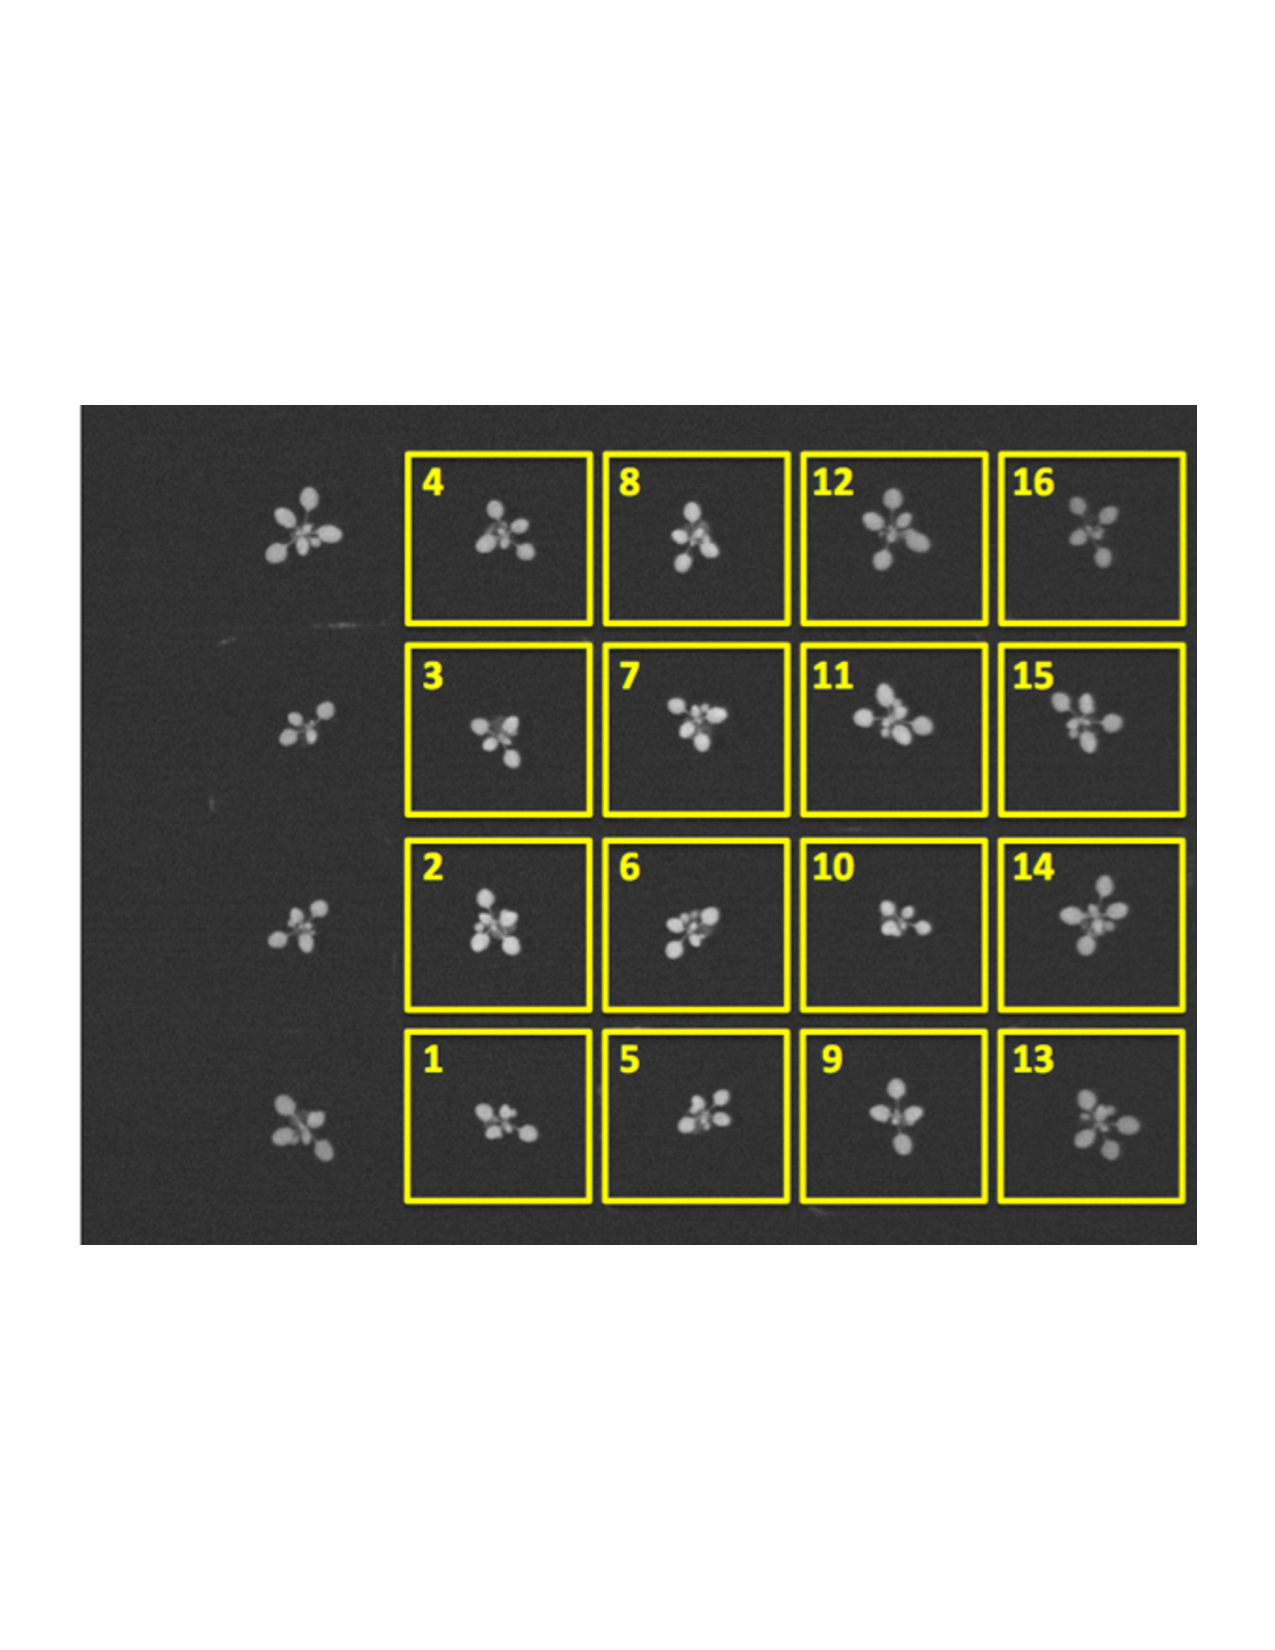
\includegraphics[width=.23\textwidth]{Figures/FourModalities/A_fmp}&
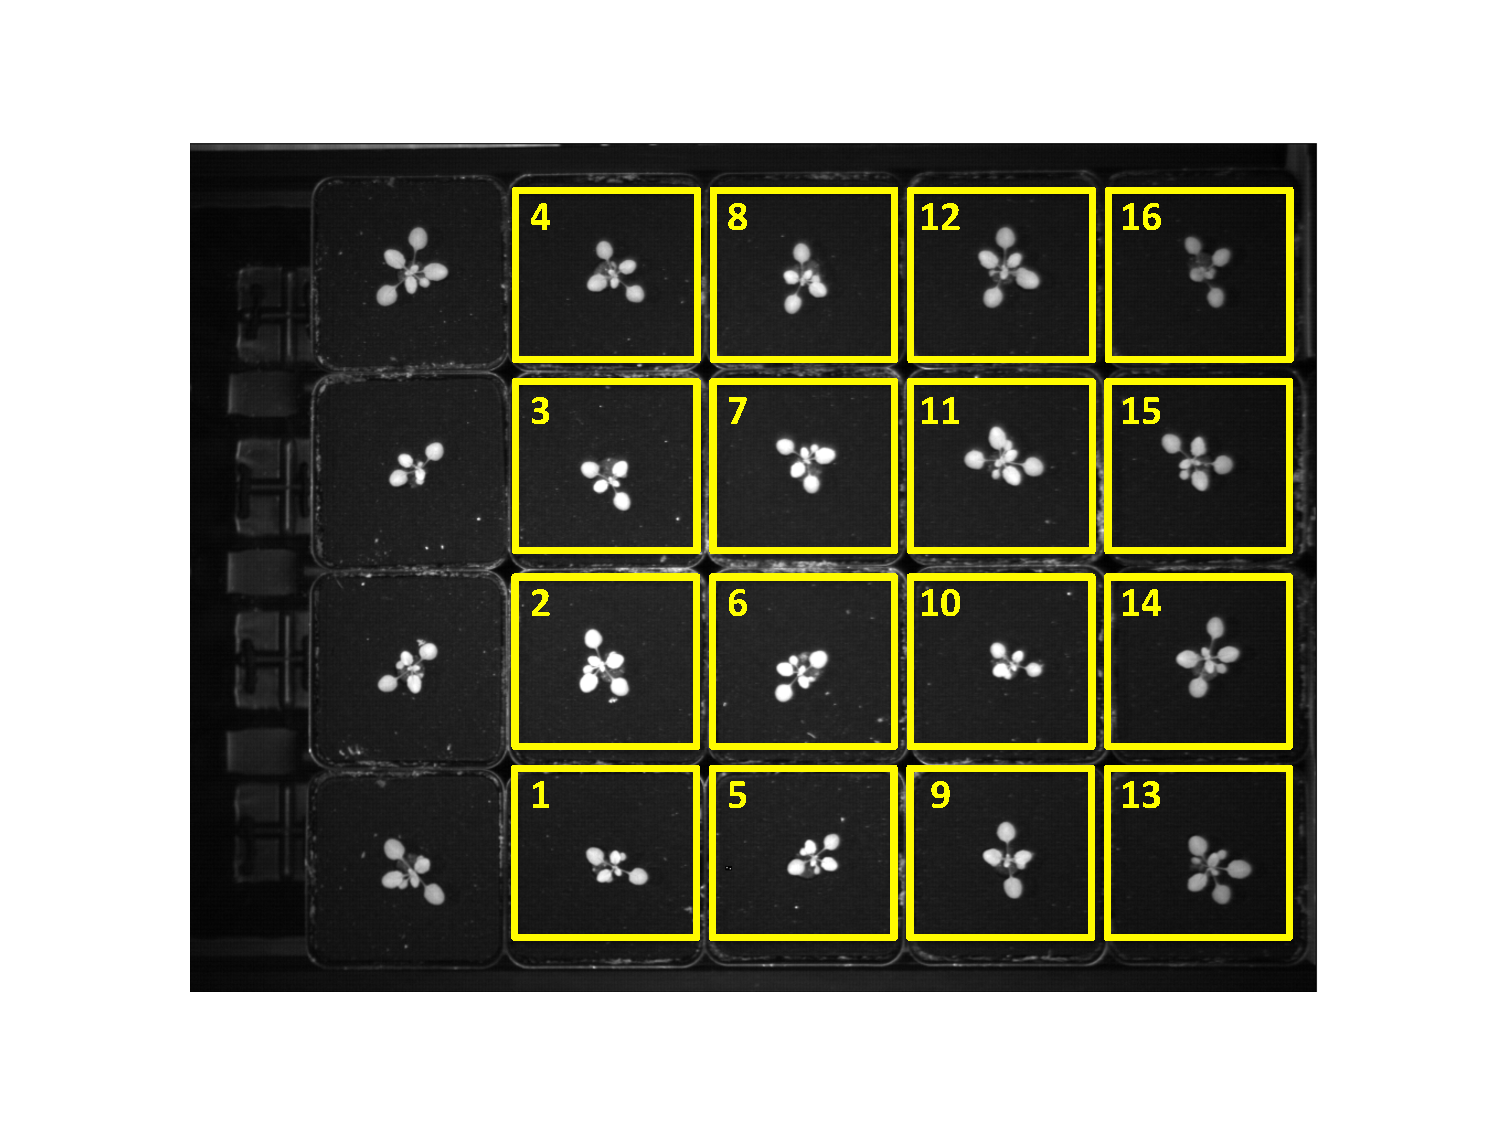
\includegraphics[width=.23\textwidth]{Figures/FourModalities/A_ir}\\
(b) &
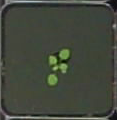
\includegraphics[width=.1\textwidth]{Figures/FourModalities/A1_rgb}&

\includegraphics[width=.1\textwidth]{Figures/FourModalities/A1_depth}&
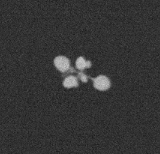
\includegraphics[width=.1\textwidth]{Figures/FourModalities/A1_fmp}&
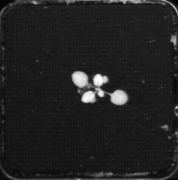
\includegraphics[width=.1\textwidth]{Figures/FourModalities/A1_ir}\\
%Arabidopsis: RGB & Arabidopsis: depth & Arabidopsis: fluorescence & Arabidopsis: IR \\
(c) &
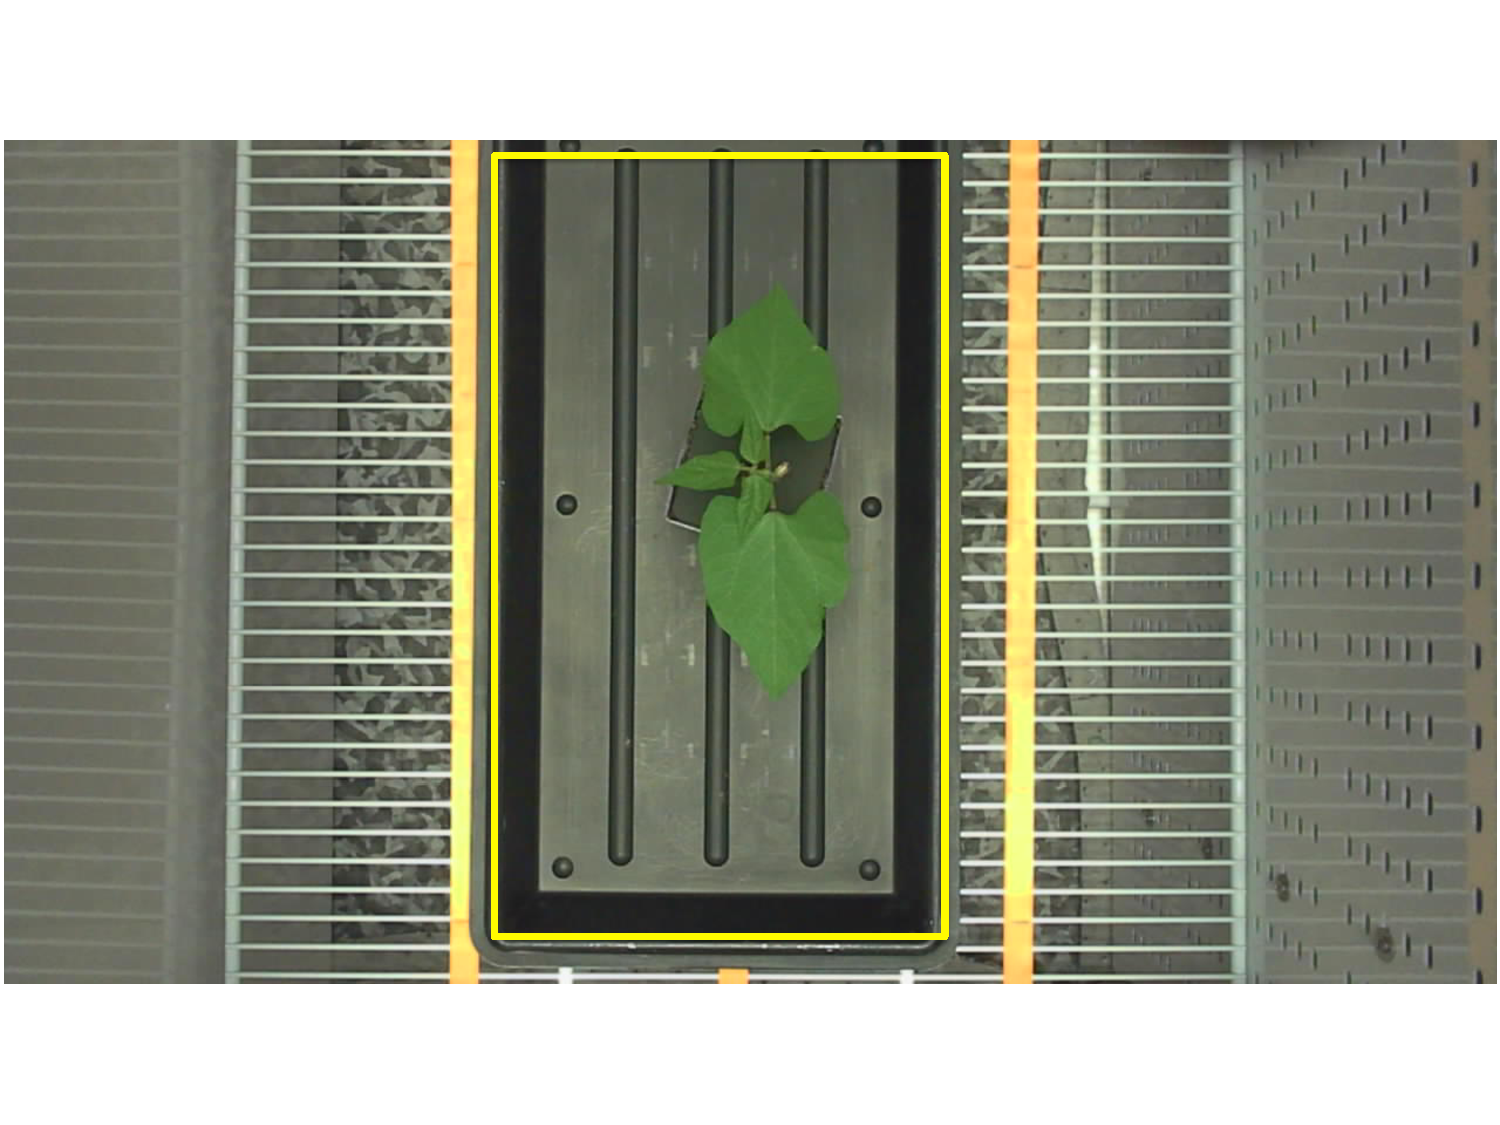
\includegraphics[width=.23\textwidth]{Figures/FourModalities/B_rgb}&
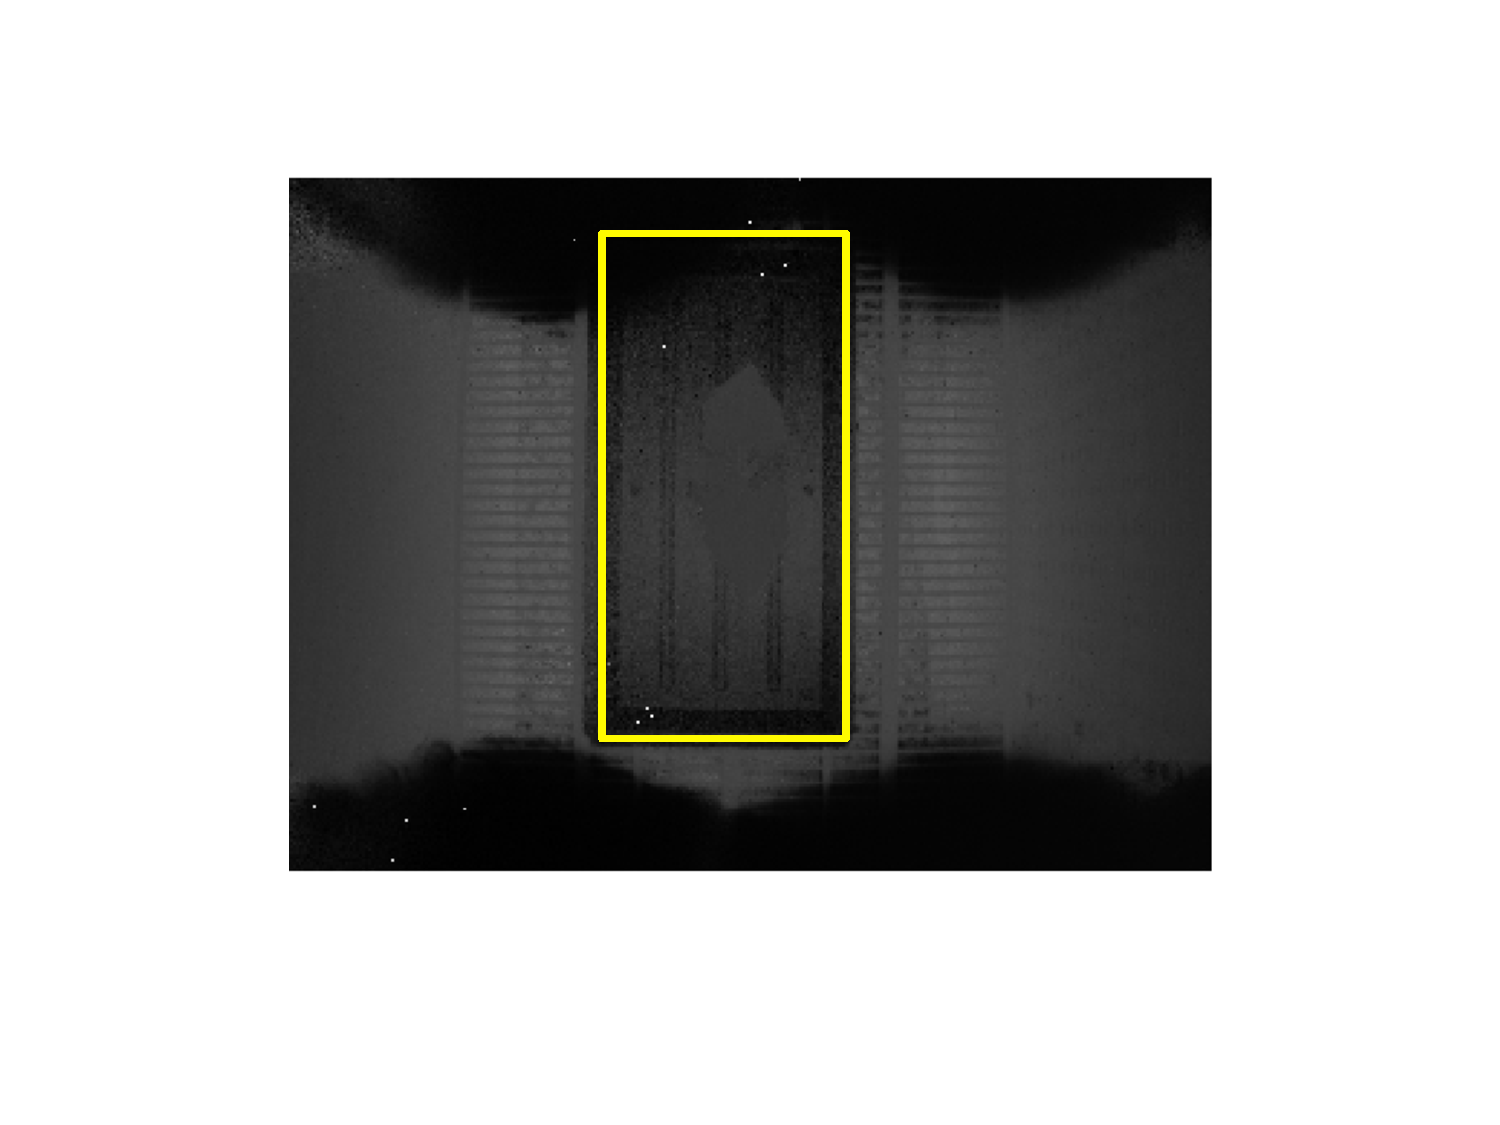
\includegraphics[width=.23\textwidth]{Figures/FourModalities/B_depth}&
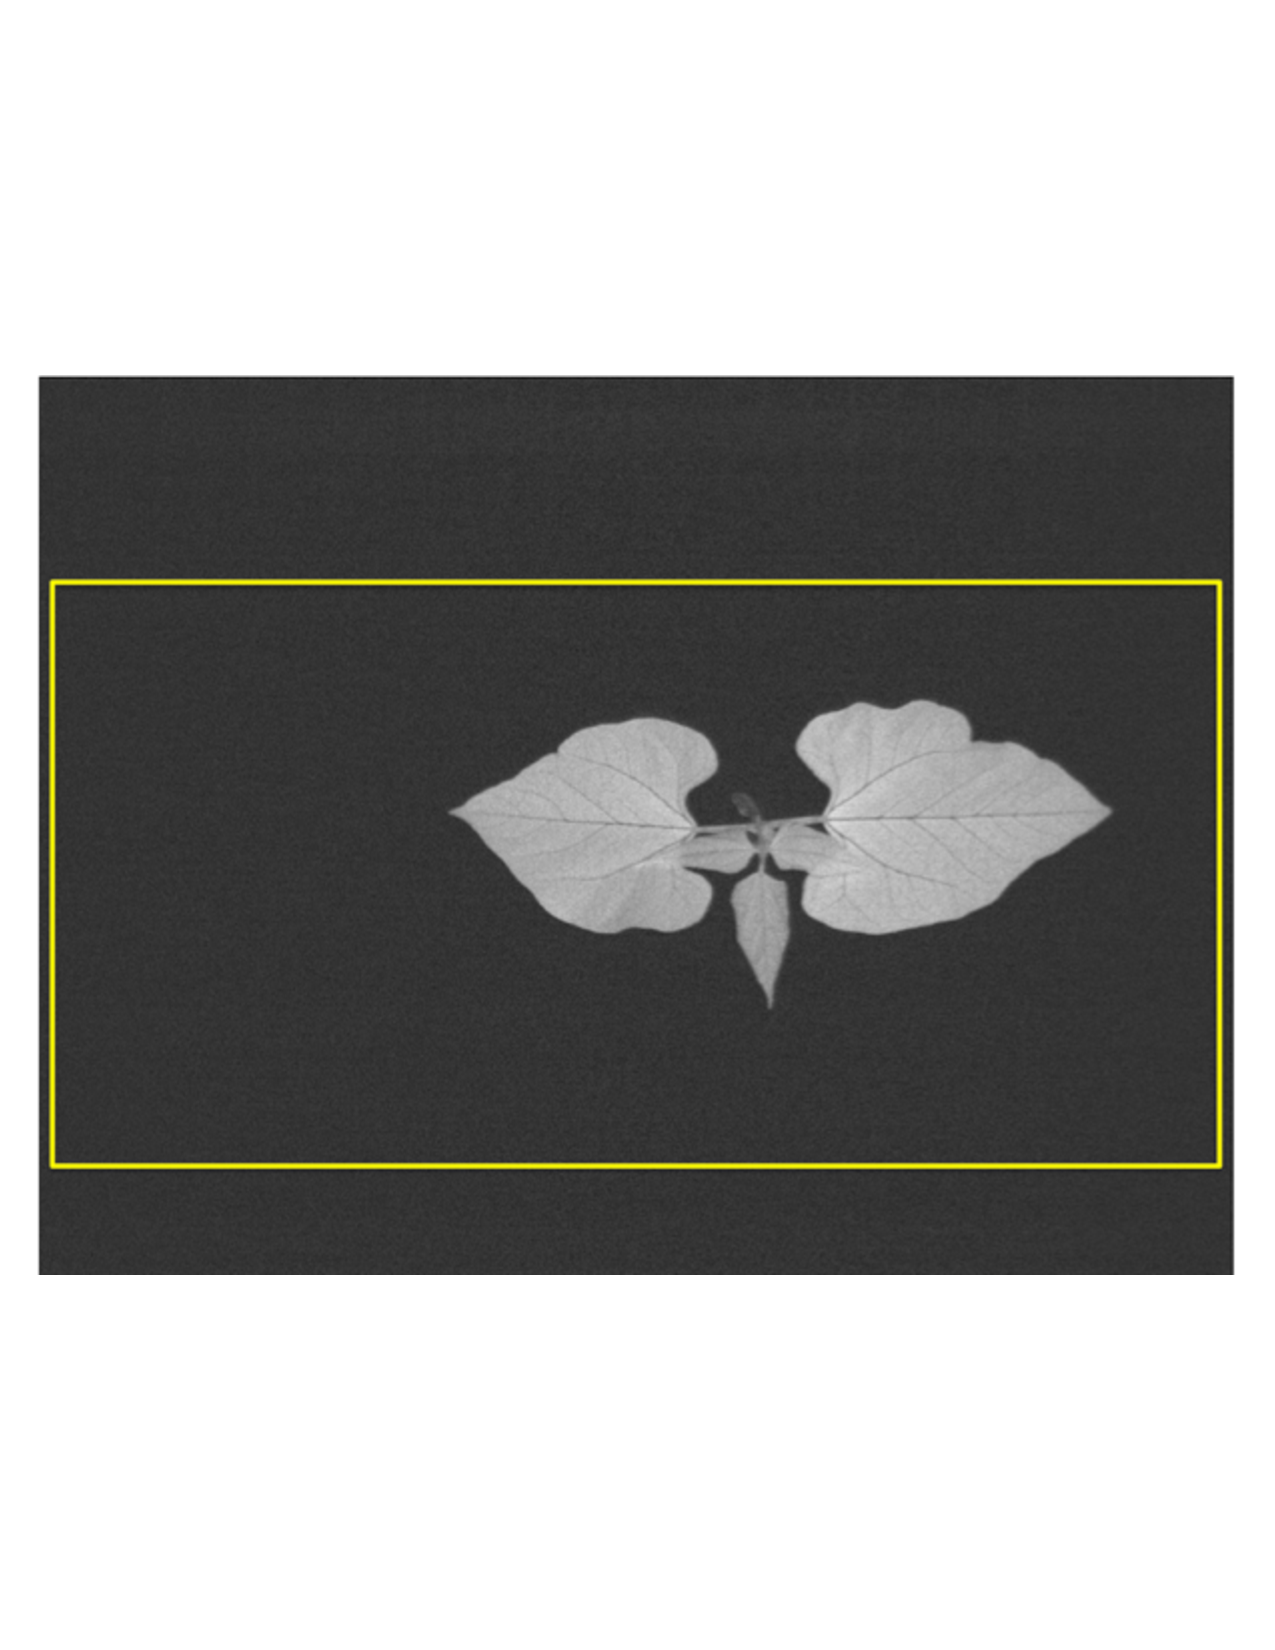
\includegraphics[width=.23\textwidth]{Figures/FourModalities/B_fmp}&
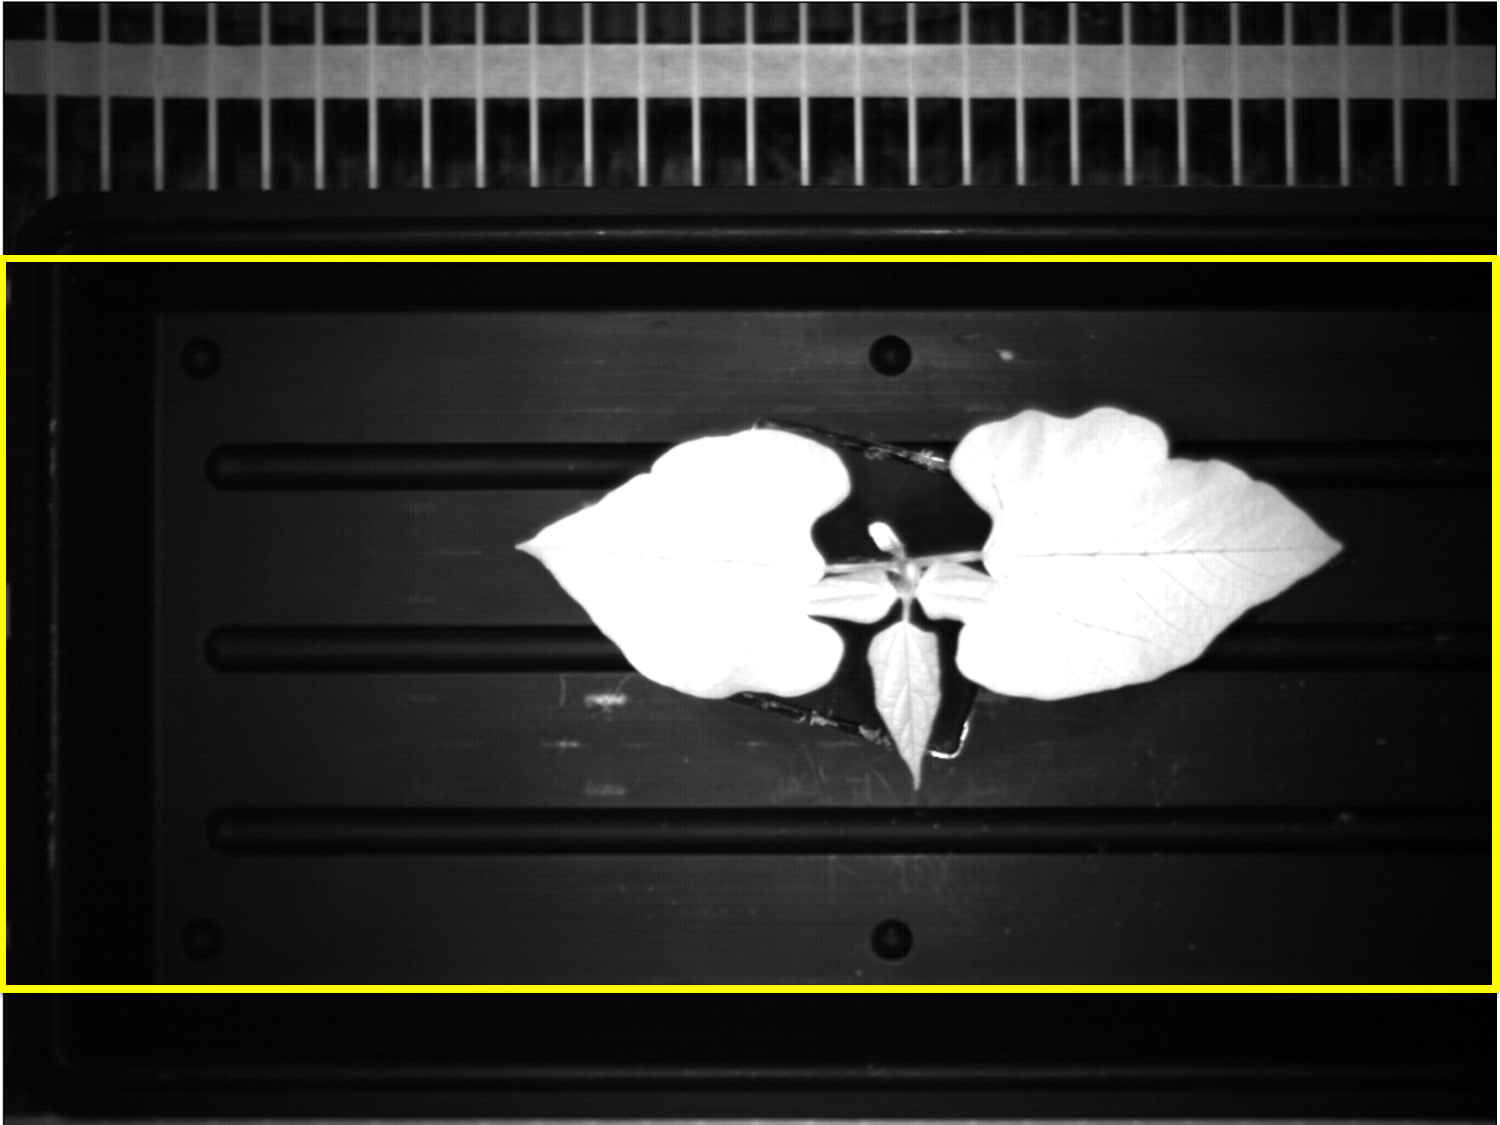
\includegraphics[width=.23\textwidth]{Figures/FourModalities/B_ir}\\
%(d) &
%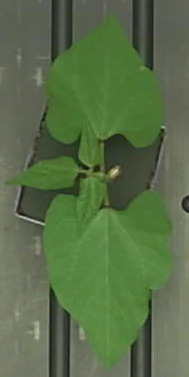
\includegraphics[width=.1\textwidth]{Figures/FourModalities/B1_rgb}&
%
\includegraphics[width=.1\textwidth]{Figures/FourModalities/B1_depth}&
%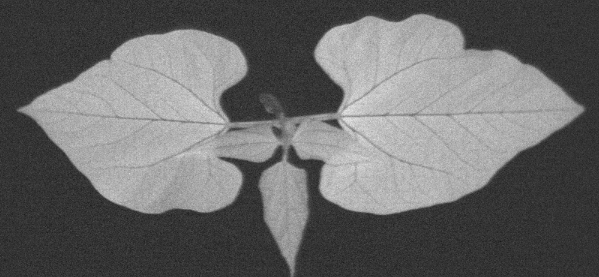
\includegraphics[width=.2\textwidth]{Figures/FourModalities/B1_fmp}&
%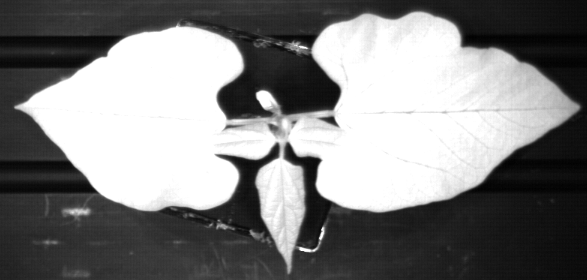
\includegraphics[width=.2\textwidth]{Figures/FourModalities/B1_ir}\\
%Bean: RGB & Bean: depth & Bean: fluorescence & Bean: IR \\
 & RGB & depth & fluorescence & IR\\
\end{tabular}
\caption{The multi-modality plant imagery database of MSU-PID. (a) four modalities of Arabidopsis; (b) zoom in view of Arabidopsis plant $1$; (c) four modalities of bean.}
\label{fig:fourmodality}
\end{centering}
\end{figure*}


Plants develop through a complex interaction between genotype and environment.
This determines their structure, functions, and thus performance such as yield or efficient usage of resources.
In order to understand the genetic basis of these economically important parameters, it is essential to quantitatively assess plant phenotypes and then identify the latent relationships to genotypes and environmental factors.
%
Plant visual phenotyping has been performed by farmers and breeders for more than $5,000$ years.
In the past, traditional phenotyping is based on experience and intuition, and is laborious~\cite{johannsenerblichkeit}.
Recent progresses in imaging sensor and computer vision technologies lead to the development of the ever-increasing new field of highly automated, non-destructive plant visual phenotyping~\cite{furbank2011phenomics,cruz2015depi}.
%Modern plant phenotyping is a comprehensive, large-scale assessment of plant traits such as growth, development, tolerance, resistance, architecture, physiology, ecology, yield, and metadata that form the basis for more complex parameters.
%
The objective of modern plant visual phenotyping is to analyze and categorize the morphological characteristics of plants, and thus accurately quantifying plant traits. %It advances crop yield improvement and enables the systematic study of the environmental plasticity of plants. %
In this interdisciplinary field, scientists employ various imaging sensors to capture plants and design advanced algorithms to automatically analyze the captured plant imagery, with the purpose of raising testable biological hypotheses to solve problems related to growth, development, stress tolerance, resistance, and so on.
%
%In old days, plant phenotyping was conducted through manual visual observation~\cite{Erblichkeit1903}. Today, motivated by the increasing lower cost and increasing diversity of imaging sensors technologies, image-based automatic plant visual phenotyping is quickly growing into a desirable and viable solution~\cite{furbank2011phenomics,cruz2015depi}.
%
A key advance in visual phenotyping is the capability to non-invasively capture plant traits, enabling continuous measurements that are necessary to monitor plants during growth and/or under stress conditions. 
It also increases the throughput of phenotyping experiments by eliminating destructive operations, which allows more genotypes or biological replicates to be examined under the same environmental conditions~\cite{fahlgren2015lights,walter2015plant}.

One goal of plant visual phenotyping is to accurately quantify plant traits, particularly those related to photosynthetic performance, growth, yield, and resilience to environmental stress.
For the approaches to be of practical, plants must be monitored continuously, over developmental time scales and under conditions that approximate the native environment (dynamic 'field' conditions)~\cite{fahlgren2015lights,walter2015plant}.
%
The capacity to identify and track individual leaves over time is important to clearly define phenotypic behaviors related to leaf-specific factors such as developmental age~\cite{schottler2015photosynthetic} and/or following the application of stress.
For example, decrease in the average photosynthetic efficiency ($\Phi_{II}$, quantum yield of photochemistry at photosystem II) of an Arabidopsis plant may reflect a heterogeneous distribution of $\Phi_{II}$ values across its entire photosynthetic surface area~\cite{oxborough2004imaging}.
In this case, mapping distributions to individual leaves can distinguish between a systemic (whole plant) effect and localization of the effect to subset leaves.
%
In addition, using more detailed information, such as leaf angles, height, and position as well as canopy density and size, it is possible to improve the estimation of total photosynthetic capacity over time (particularly for plants with more complex canopies, e.g., common bean or tobacco), since these factors influence absorption and availability of the light energy used to drive photosynthesis.

\begin{table*}[t!]
\centering
\begin{threeparttable}
\caption{Plant image databases.}
%\resizebox{12cm}{!} {
%\begin{tabular}{|l@{}|@{}c@{}|@{}c@{}|@{}c@{}|@{}c@{}|@{}c@{}|}
\begin{tabular}{l|c|c|c|c|c|c}
%\hline
%\multirow{2}{*}{Database}& \multirow{2}{*}{Modality} & \multirow{2}{*}{Applications}\tnote{a} & \multirow{2}{*}{Plant Type} & Subject/ &Total & Labeled \\
%& & & & Classe \# & Image \# & Image \# \\ \hline
%Swedish leaf~\cite{soderkvist2001computer} & Scaned leaf & LC& Swedish trees & $15$ & $1,125$ & $1,125$ \\ \hline
%Flavia~\cite{wu2007leaf} & RGB & LC& Leaves & $32$ & $2,120$ & $2,120$ \\ \hline
%Leafsnap~\cite{kumar2012leafsnap} & RGB & LC& USA trees & $184$ & $29,107$ & $29,107$ \\ \hline
%Crop/weed~\cite{haug2014crop} & RGB &Weed detection & Crop/weed & $2$ & $60$ & $60$ \\ \hline
%\multirow{2}{*}{LSC~\cite{haug2014crop}} & \multirow{2}{*}{RGB} & \multirow{2}{*}{LS, LO} & Arabidopsis & $43$ & $6287$ & $201$ \\ \cline{4-7}
%& & & Tobacco & $80$ & $165,120$ & $83$ \\ \hline
%\multirow{2}{*}{MSU-PID} & fluorescence, & LS, LO, & Arabidopsis & $16$ & $2304\times 4$ & $576\times 4$ \\ \cline{4-7}
%& IR, RGB, depth & LA, LT & Bean & $5$ & $350\times 4$ & $175\times 4$ \\ \hline
%\hline
\hline
\multirow{2}{*}{Database}& \multirow{2}{*}{Modality} & \multirow{2}{*}{Applications}\tnote{a} & \multirow{2}{*}{Plant Type} & Subject/ &Total & Labeled \\
& & & & Classe \# & Image \# & Image \# \\ \hline
Swedish leaf & \multirow{2}{*}{Scaned leaf} & \multirow{2}{*}{LC} & \multirow{2}{*}{Swedish trees} & \multirow{2}{*}{$15$} & \multirow{2}{*}{$1,125$} & \multirow{2}{*}{$1,125$} \\
~\cite{soderkvist2001computer} & & & & & & \\ \hline
Flavia & \multirow{2}{*}{RGB} & \multirow{2}{*}{LC} & \multirow{2}{*}{Leaves} & \multirow{2}{*}{$32$} & \multirow{2}{*}{$2,120$} & \multirow{2}{*}{$2,120$} \\
~\cite{wu2007leaf} & & & & & & \\ \hline
Leafsnap & \multirow{2}{*}{RGB} & \multirow{2}{*}{LC} & \multirow{2}{*}{USA trees} & \multirow{2}{*}{$184$} & \multirow{2}{*}{$29,107$} & \multirow{2}{*}{$29,107$} \\
~\cite{kumar2012leafsnap} & & & & & & \\ \hline
Crop/weed & \multirow{2}{*}{RGB} & \multirow{2}{*}{Weed detection} & \multirow{2}{*}{Crop/weed} & \multirow{2}{*}{$2$} & \multirow{2}{*}{$60$} & \multirow{2}{*}{$60$} \\
~\cite{haug2014crop} & & & & & & \\ \hline
LSC & \multirow{2}{*}{RGB} & \multirow{2}{*}{LS, LO} & Arabidopsis & $43$ & $6,287$ & $201$ \\ \cline{4-7}
~\cite{haug2014crop} & & & Tobacco & $80$ & $165,120$ & $83$ \\ \hline
\multirow{2}{*}{MSU-PID} & fluorescence, & LS, LO, & Arabidopsis & $16$ & $2,160\times 4$ & $576\times 4$ \\ \cline{4-7}
& IR, RGB, depth & LA, LT & Bean & $5$ & $325\times 4$ & $175\times 2$ \\ \hline
\hline
\end{tabular}
%}
\begin{tablenotes}
\footnotesize
\item[a] The abbreviation in ``Applications'' column is defined as Leaf Classification (LC), Leaf Segmentation (LS), Leaf Counting (LO), Leaf Alignment (LA), and Leaf Tracking (LT).
\end{tablenotes}
\end{threeparttable}
\label{tab:database}
\end{table*}

Due to diverse variations of leaf shape, appearance, layout, growth and movement, plant image analysis is a non-trivial computer vision task~\cite{Minervini2015}.
In order to develop advanced computer vision algorithms, image databases that are well representative of this application domain is highly important.
In fact, computer vision research lives on and advances with databases, as evidenced by the successful databases in the field (e.g., FERET~\cite{Phillips2000} and LFW~\cite{LFW}).
However, the publicly available databases for plant phenotyping are still very limited, with the only exception of LSC database~\cite{scharr2014annotated}, which, nevertheless, has its own limitations on the type of images (RGB only) and is only suitable for a small set of plant image analysis applications.


To facilitate future research on plant image analysis, as well as remedy the limitation of existing databases in the field, this paper presents a newly collected multi-modality Plant Imagery Database through an interdisciplinary effort at Michigan State University (MSU), which is termed ``MSU-PID''.
As illustrated in Figure~\ref{fig:fourmodality}, the MSU-PID database includes the imagery of two types of plants (Arabidopsis and bean, both are widely used in plant research) captured by four types of imaging sensors, i.e., fluorescence, infrared (IR), RGB color, and depth.
All four sensors are synchronized and are programmed to periodically capture imagery data for multiple consecutive days.
Checkerboard-based camera calibration is performed on each modality providing intrinsic camera parameters and poses.  In addition explicit correspondence between the pixels of {\it any} two modalities is obtained using an homographic warping of a plane through the Arabidopsis plants.


The type and amount of manual labels on a database is a critical enabler to the potential applications of the database.
For a subset of the MSU-PID database, we manually label the groundtruth regarding the leaf identification number, locations of leaf tips, and leaf segments.
As a result, MSU-PID is suitable for a number of applications, including $1)$ {\it leaf segmentation} that aims at estimating the correct segmentation mask of each leaf in an image, $2)$ {\it leaf counting} that estimates the correct number of leaves within a plant, $3)$ {\it leaf alignment} that aligns the two tips of each leaf -- the cornerstone of the leaf structure, and $4)$ {\it leaf tracking} that is designed to track each leaf over time.
Finally, to provide a performance baseline for future research and comparison, we apply our automatic leaf segmentation framework~\cite{yin2014a,yin2014b} to the Arabidopsis imagery and demonstrate the unique challenge of image analysis on this database.

In summary, this paper and our database have made the following main contributions.
\begin{itemize}
\item MSU-PID is the first {\it multi-modality} plant image database. This allows researchers to study the strength and weakness of individual modality, as well as their various combinations in plant image analysis.
\item Our unique imaging setup and the variety of manual labels make MSU-PID an ideal candidate for evaluating a diverse set of plant image analysis applications including leaf segmentation, leaf counting, leaf alignment, leaf tracking, and potentially leaf growth prediction and $3$D leaf reconstruction.
\end{itemize}




\section{Prior Work}
\label{sec:prior}

Databases drive computer vision research.
Hence, it is always important to develop and promote properly captured databases in the vision community.
While there is a clear desire to apply computer vision to plant image analysis, the lack of publicly available plant image databases has been an obstacle for further study and development.

We summarize existing publicly available databases that are most related to our work in Table~\ref{tab:database}.
In terms of potential applications of these databases, they can be categorized into two types.
The first type is for the general purpose of recognizing a particular species of tree or plant.
The Swedish leaf database~\cite{soderkvist2001computer} is probably the first leaf database even though the images are captured by scanners.
The Flavia database~\cite{wu2007leaf} is considerably larger and a neural network is utilized to train a leaf classifier.
The most recent Leafsnap project~\cite{kumar2012leafsnap} is an impressive effort that includes a very large dataset of leaves for $184$ tree types.
A mobile phone application is also developed to make the leaf classification system portable.
Finally, the crop/weed image database~\cite{haug2014crop} is captured by a robot in the real field, and used for the classification of crop vs. weed.
Note that except for~\cite{haug2014crop} where images are captured in the wild for a large area of plant, other databases in this type normally capture only a {\it single} leaf in a relatively constrained imaging environment.
Therefore, the challenging problem of leaf segmentation has been bypassed.
% Note that in this type of databases, normally only a {\it single} leaf is imaged in a relatively constrained imaging environment and as a result, the challenging problem of leaf segmentation has been bypassed.

The second type of databases is for plant phenotyping, where it is important to capture plant images without interfering the growth of plants.
Thus, non-destructive imaging approaches are taken and the entire plant is imaged. 
The LSC database~\cite{scharr2014annotated} is the most relevant one to our database.
It captures a large set of RGB images for Arabidopsis and tobacco plants.
The provided manual labels allow the evaluation of leaf segmentation and leaf counting.
In comparison, our MSU-PID database utilizes four sensing modalities in the data capturing, each providing different aspects of plant visual appearance.
Our diverse manual labels also enable us to develop algorithms for additional applications such as leaf tracking and leaf alignment.

%One of our data modalities is dense depth measurement. This has been a component of a number of recent non-plant RGB-D databases designed for object recognition~\cite{Lai2011}, scene segmentation~\cite{Silberman2011}, human analysis~\cite{Sung2011,Barbosa:reid12}, and mapping~\cite{sturm12iros}. By including dense depth for a plant database we anticipate enabling development of new 3D plant shape analysis algorithms.

The four sensing modalities in MSU-PID provide unique opportunities to comprehensively characterize plant morphological and physiological phenotypes. 
The use of chlorophyll fluorescence at $730nm$ to $750nm$ as a tool for evaluating photosynthetic performance is well established~\cite{baker2008chlorophyll}, and against non-(chlorophyll)fluorescent background clearly defines photosynthetically active leaf area.
The depth measurement has been a component of a number of recent non-plant RGB-D databases designed for object recognition~\cite{Lai2011}, scene segmentation~\cite{Silberman2011}, human analysis~\cite{Sung2011,Barbosa:reid12}, and mapping~\cite{sturm12iros}. 
By including depth map for a plant database, we anticipate enabling development of new $3$D plant canopy analysis algorithms and thus probing the total energy intake and storage.
Near infrared (IR) reflectance has been used by others to detect water content in leaves~\cite{chen2014dissecting}.  
However, it may also be useful in determining leaf angle and curvature.  
Furthermore, since imaging occurs at a wavelength that is effectively non-absorbing for photosynthesis or known light receptors~\cite{butler1964actton,eskins1992light} in plants, it can be used for imaging during the night cycle to observe night time leaf expansion or in some cases circadian movements~\cite{mcclung2006plant}.








\section{Data Collection}
\label{sec:2}

\subsection{Plants and Growth Conditions}

{\it Arabidopsis thaliana} (ecotype Col-$0$) plants were grown at $20^{\circ}C$, under a $16~hr$ : $8~hr$ day-night cycle with a daylight intensity set at $100~\mu mol~photons~m^{-2} s^{-1}$.
%
Black bean plants ({\it Phaseolus vulgaris L.}) of the cultivar Jaguar, were grown under a $14~hr$ : $10~hr$ day-night cycle with day and night temperatures of $24^{\circ}C$ and $18^{\circ}C$ respectively, and a daylight intensity set at $200~\mu mol~photons~m^{-2} s^{-1}$.
%
Note that the bean plants were watered with half-strength Hoaglands solution three times per week.

In all cases, seeds were planted in soil covered with a black foam mask in order to minimize the fluorescence background from algal growth.
%
Two-week-old plants ({\it Arabidopsis} and bean) were transferred to imaging chambers and allowed to acclimate (\todo{Jeff: Please define ``acclimate" as in Comment $37$}) for $24$ hours to the LED lighting before the start of the data collection.
Growth conditions as described above were maintained for each set of plants for the duration of image collection.


\begin{figure}
  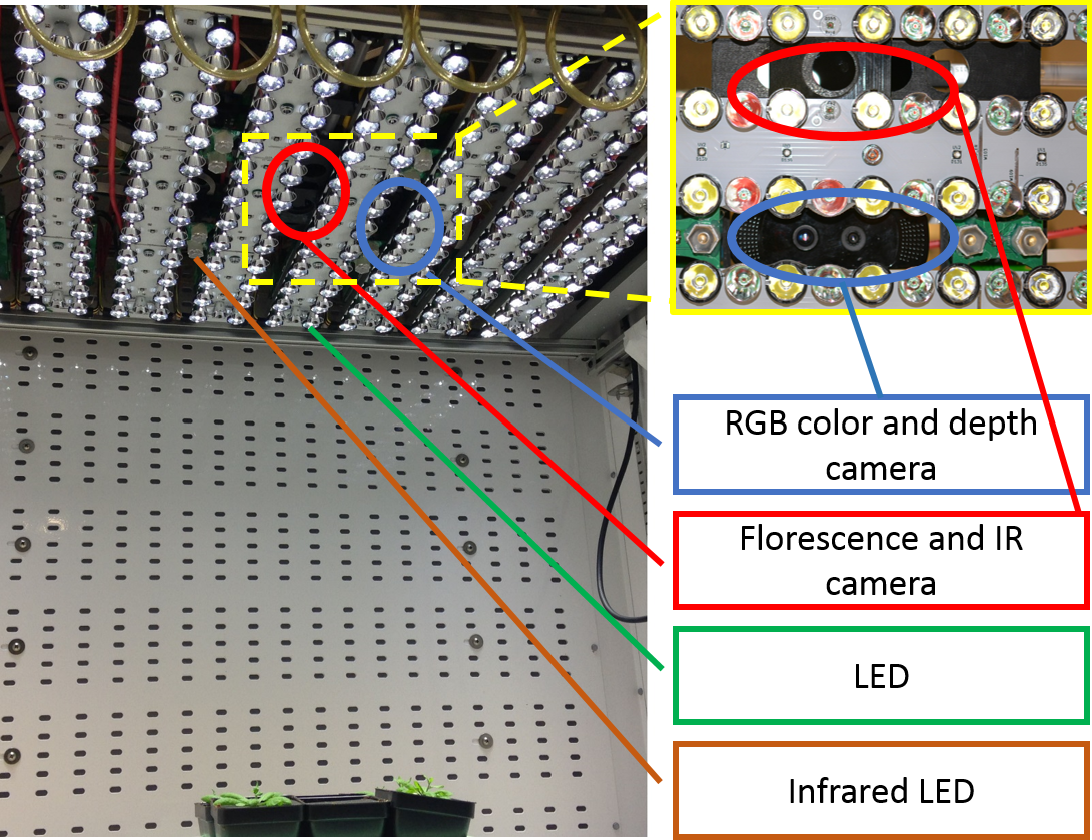
\includegraphics[width=\linewidth,trim=55 100 200 70,clip]{Figures/hardware}
\caption{The hardware setup for our data collection.}
\label{fig:hardware}
\end{figure}

\subsection{Hardware Setup}

In this section, we introduce the hardware used for capturing fluorescence, IR, RGB color, and depth imagery data for both plants.
Figure~\ref{fig:hardware} illustrates the hardware and imaging setup used in our data collection.

\subsubsection{Fluorescence and IR Images}
Chlorophyll a fluorescence images were captured once every hour during the daylight period in a growth chamber~\cite{cruz2015depi}.
A set of $5$ images were captured using a Hitachi KP-F145GV CCD camera (Hitachi Kokusai Electric America Inc., Woodbury, NY) outfitted with an infrared long pass filter (Schott Glass RG-9, Thorlabs, Newton, NJ), during a short period ($<400~ms$) of intense light saturating to photosynthesis ($>10,000~\mu mol~photons~m^{-2} s^{-1}$) provided by an array of white Cree LEDs (XMLAWT, 5700K color temperature, Digi-Key, Thief River Falls, MN) collimated using a $20~mm$ Carclo Lens (10003, LED Supply, Lakewood, CO).
%
Chlorophyll a fluorescence was excited using monochromatic red LEDs (Everlight $625~nm$, ELSH-F51R1-0LPNM-AR5R6, Digi-Key), collimated using a Ledil reflector optic ($C11347\_REGINA$, Mouser Electronics, Mansfield, TX) and pulsed for $50~\mu s$ during a brief window when the white LEDs were electronically shuttered.
In addition, a series of $5$ images were also collected in the absence of the excitation light for artifact subtraction.

Infrared images were collected once every hour with the same camera and filter used for chlorophyll a fluorescence.
Pulses of $940~nm$ light were provided by an array of OSRAM LEDs (SFH 4239, Digi-Key), collimated using a Polymer Optics lens (Part no. 170, Polymer Optics Ltd., Berkshire, England).
Since $940~nm$ light does not influence plant development or drive photosynthesis, images were also collected during the night period.
Sets of $15$ images were collected for averaging, in the absence of saturating illumination.
As with chlorophyll a fluorescence, images were captured in the absence of $940~nm$ light for artifact subtraction.



\subsubsection{RGB Color and Depth Images} %This section describes characterizes the data from this sensor, particularly the depth data.

The RGB color and depth images were collected using a Creative Senz3D sensor~\cite{nguyen2015vietnamese}. The sensor contains both a $1280 \times 720$ color camera directed parallel to, and separated by roughly $25~mm$ from, a depth camera which has a resolution of $320\times240$ pixels.
The depth sensor uses a flash near IR illuminator and measures the time-of-flight of the beam at each pixel to obtain dense depth estimates along with an IR reflectance at each pixel.

There are a number of limitations to the depth sensor that become the sources of depth errors.
The primary measurement limitation on the range-to-target is the strength of the reflected beam.
As a result, dark, matt surfaces are measured reliably only at a close range on the order of $20$ or $30~cm$.
Highly reflective surfaces also pose problems with direct reflections leading to saturation and highly unreliable depths.
In addition reflective surfaces at grazing angles are less reliably measured since little signal is reflected.
Fortunately the primary goal of the depth measurements are to obtain leaf depths, and plants provide good, roughly Lambertian, reflections of IR~\cite{Chelle2006219}.  Thus the depth pixels that are most reliable and are of most use are those that fall on plant foliage.

% For one-column wide figures use
\begin{figure}
\begin{tabular}{c}
  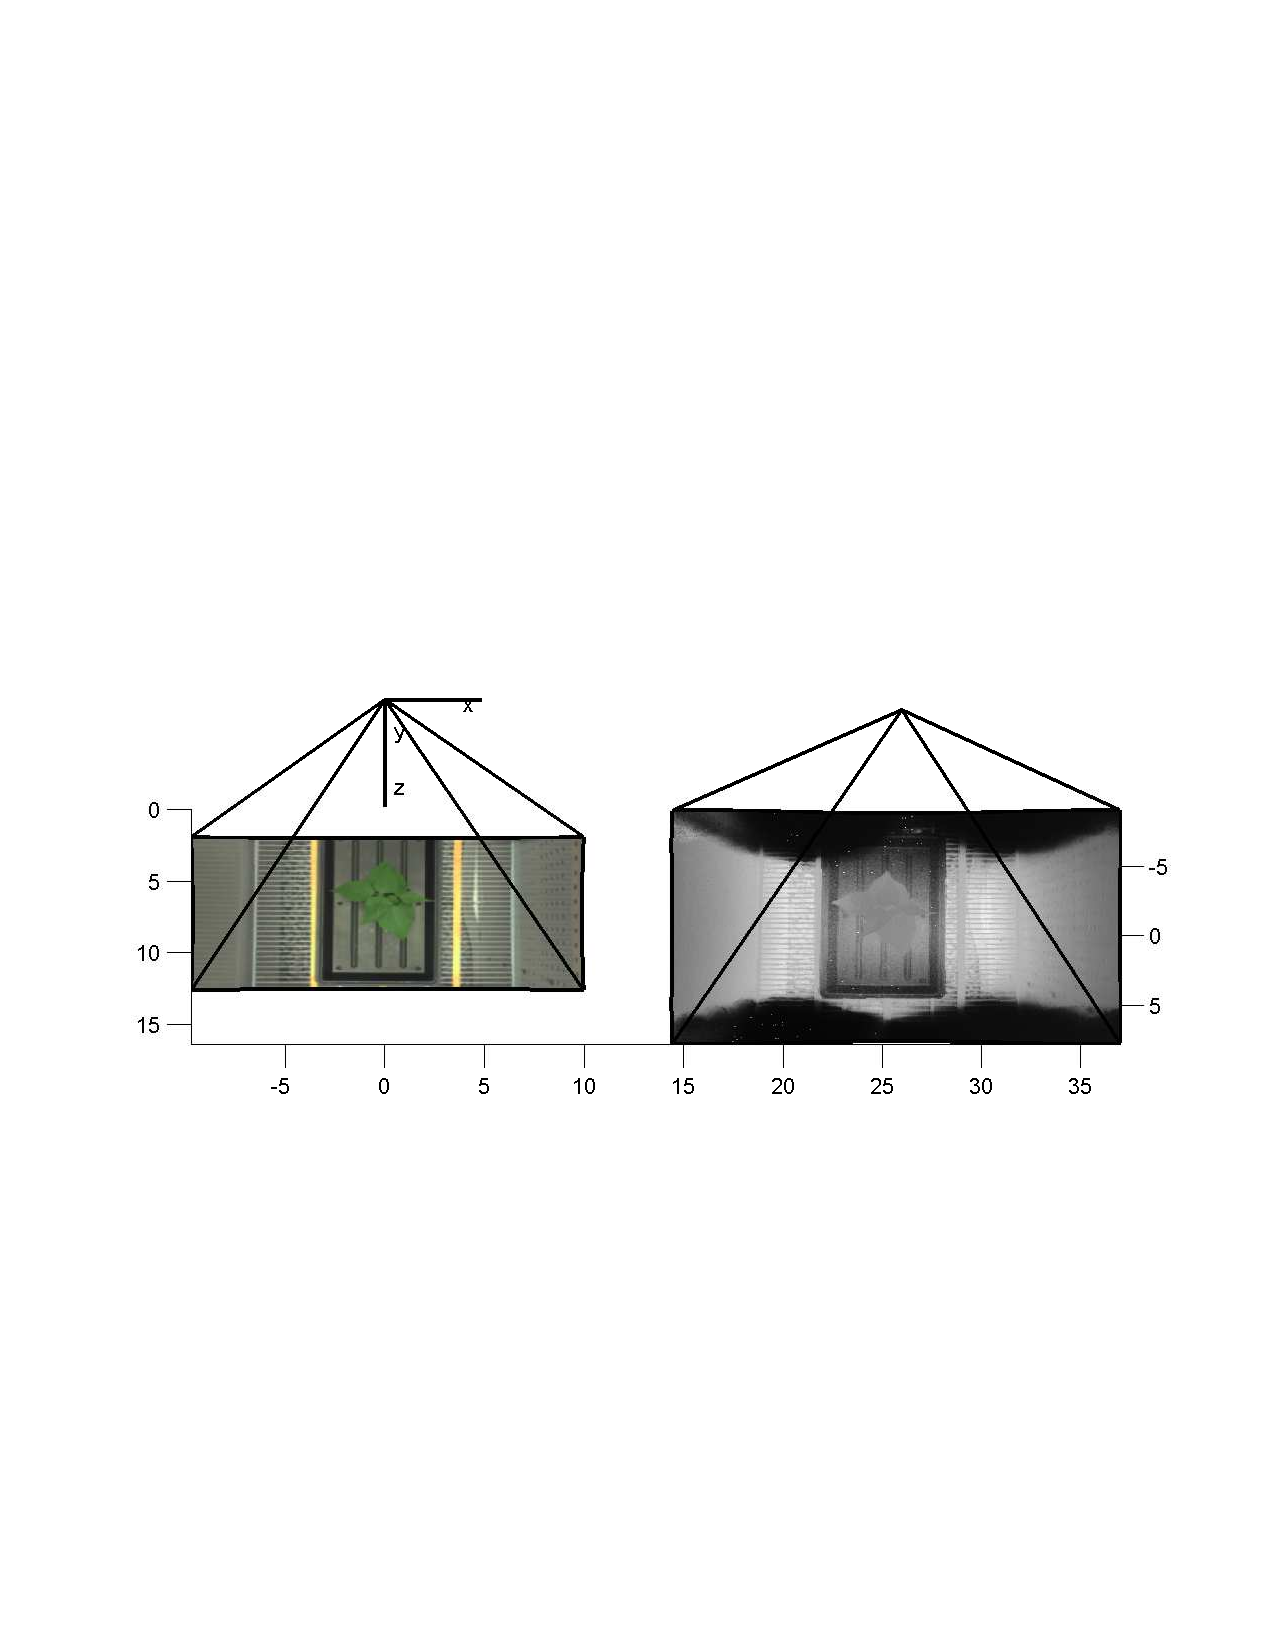
\includegraphics[width=\linewidth,trim=120 240 80 300,clip]{Figures/CameraConfiguration} \\
  ($a$)\\
  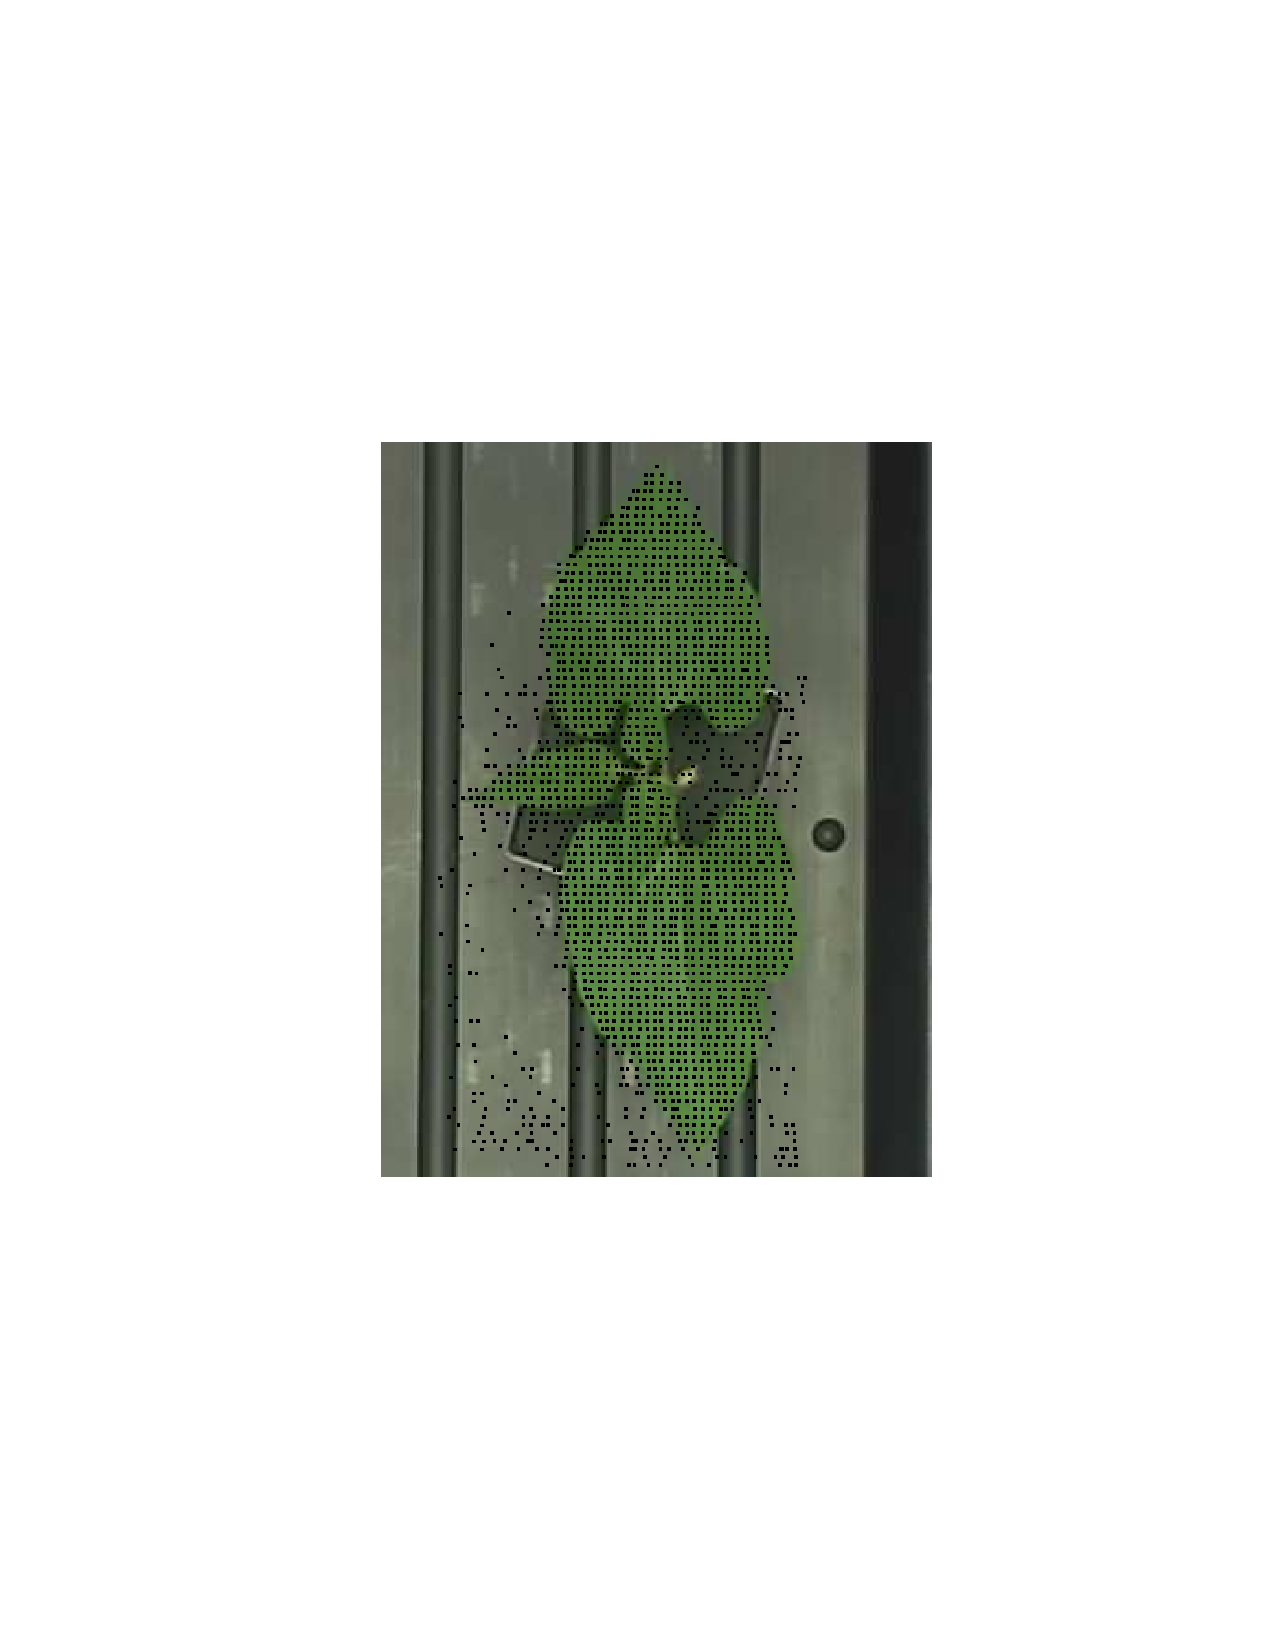
\includegraphics[width=0.65\linewidth,trim=175 220 162 180, clip,angle=-90,origin=c]{Figures/DepthOnBeanRGB} \vspace{-10mm} \\
  ($b$)\\
\end{tabular}
\caption{($a$)A plot of the three cameras showing their relative configuration and fields of view as obtained through calibration.  Units are in $mm$, apart from the size of the images which are scaled and plotted at equal resolution.  The optical center of the color camera (left-most) defines the world coordinate system.  Close to it is the depth camera having much lower resolution.  The right-most camera is the combined fluorescent and IR camera. ($b$) $3$D points from the depth camera are projected along their rays into the world coordinates and then projected into the color and fluorescent camera images.  This shows the projection into the color image (with $90^{\circ}$ rotation for economical use of space).  Only points in a rectangular region around the plant in the depth image are selected, and these are further filtered by eliminating points with high standard deviation.  An algorithm requiring only $3$D points on the plant could select only those that fall on the leaf pixels.}
\label{fig:CameraConfiguration}
\end{figure}

The imagery data were collected once every hour.
These include the fluorescent image, the IR reflectance image with the same camera, the color image, the $3$D depth and a confidence image.
The $3$D depth image is built from the depth sensor by transforming the points into the world coordinates and is expressed in the unit of $mm$.
The confidence image is the standard deviation of the depth pixels.
This is useful for identifying pixels at depth discontinuities that are unreliably detected and result in large standard deviations.


\begin{figure}
\centering
  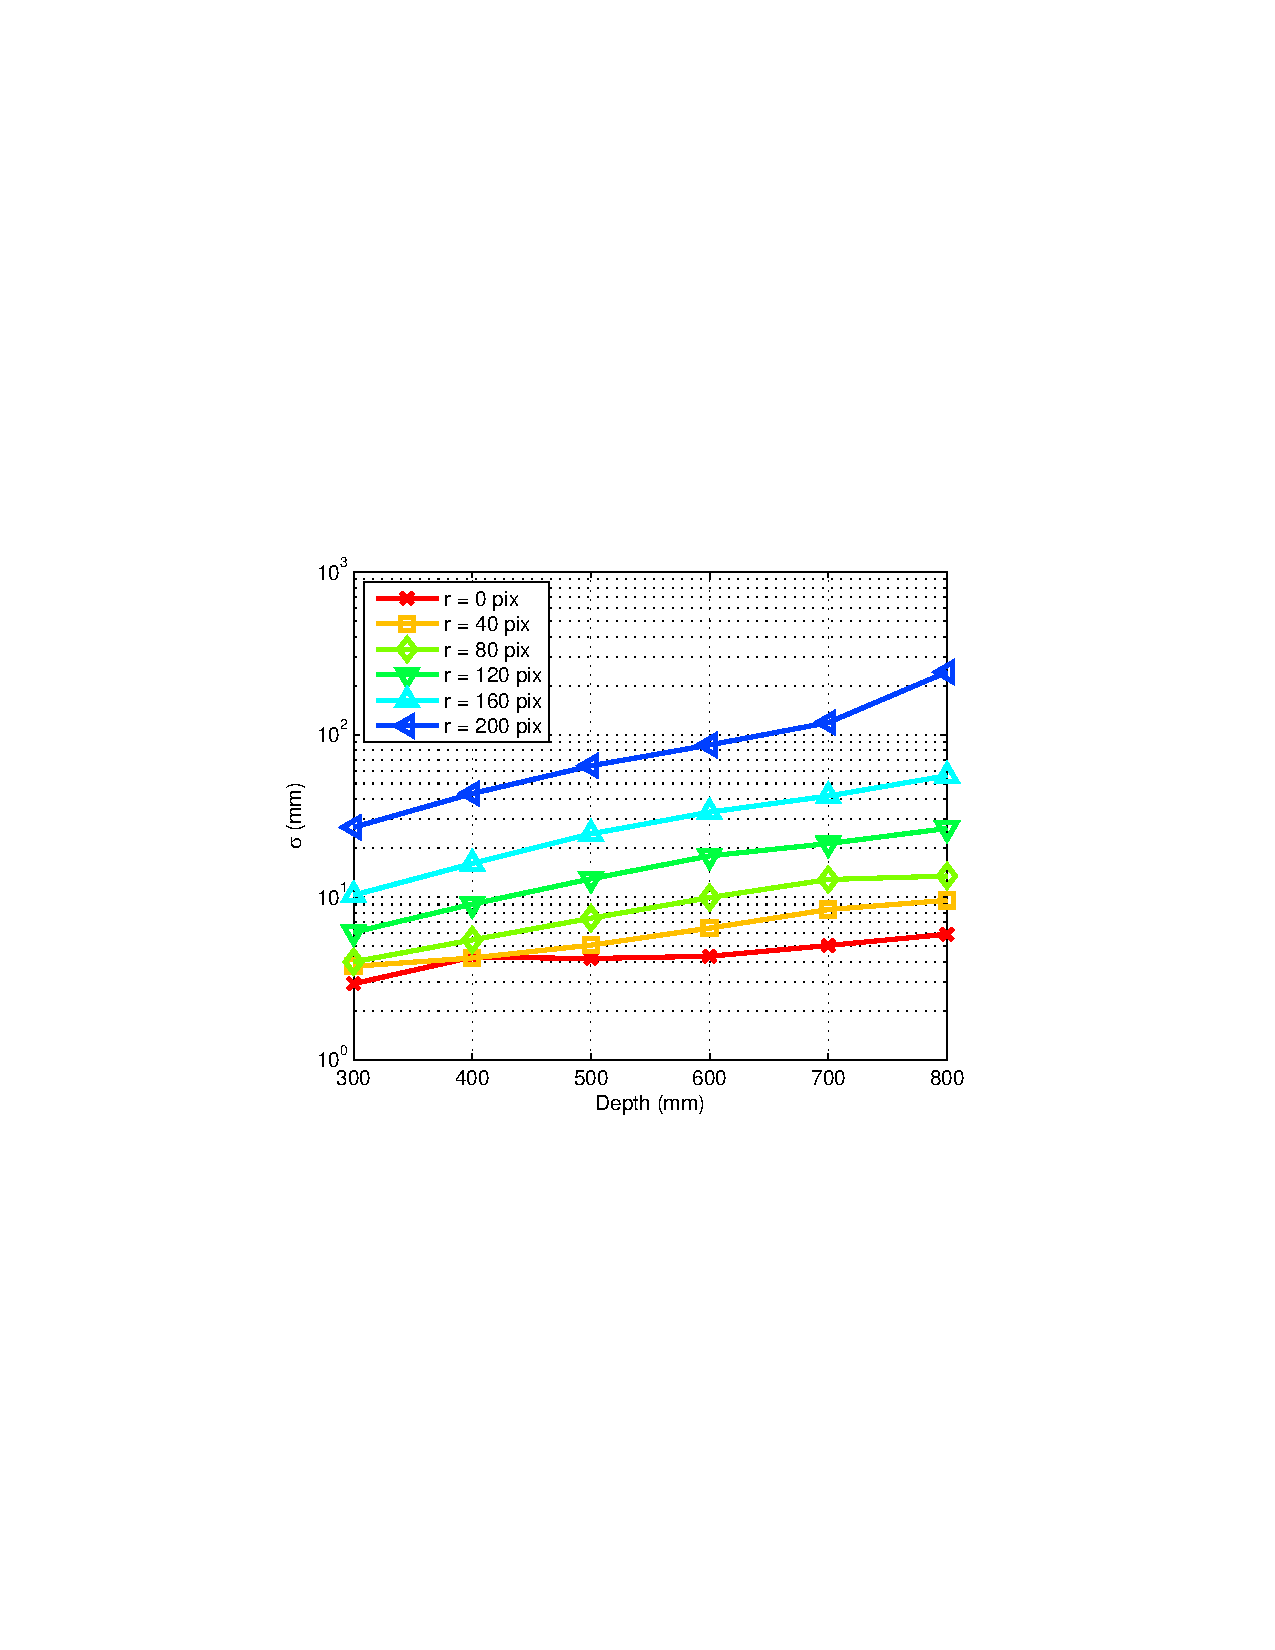
\includegraphics[height=5.9cm,trim=110 250 60 260,clip]{Figures/SigmaRadius} \\
\caption{Noise analysis for a depth camera obtained by imaging a flat surface at various depths.  We found that the standard deviation, $\sigma_I(d,r)$ from Eq. (\ref{eq:sigma}) of the pixel depth measurements had a large dependency on both the target depth, $d$, and the pixel radius, $r$, from the image center, and these are plotted.  A radius of $0$ pixels is the image center, and of $200$ pixels corresponds to the corners of the depth camera, which can be seen to have far larger standard deviation than at the image center for the same depth. }
\label{fig:Noise}
\end{figure}





\subsection{Sensor Calibration}

A planar checkerboard pattern was used to calibrate all three cameras to obtain both intrinsic and extrinsic parameters. While the grid pattern is not visible in the depth image, it is nevertheless observed in the reflected IR image whose pixels correspond to the depth pixels. This enables the use of Zhang's method~\cite{Zhang2000} to calculate the intrinsic parameters including a $2$-parameter radial distortion of each camera. In this process the poses of all three cameras are also calculated relative to the checkerboard. The intrinsic and extrinsic parameters are stored as text files, and a Matlab function is provided that reads the parameters and can plot the camera poses as in Figure~\ref{fig:CameraConfiguration}.


\subsubsection{Noise Characterization}
\label{sec:bias}

The time of flight depth measurements can have significant noise, and it is useful to both model it and quantify it. Doing so can lead to strategies to reduce noise as well as providing guidance to algorithms that use the depth measurements. Our goal in this section is to provide a simple noise model that can predict the empirically observed depth noise on smooth, Lambertian surfaces, such as plant leafs.

The depth noise, $\varepsilon$, is modeled as the sum of an image dependent term, $\varepsilon_I$, and a sensor dependent term, $\varepsilon_S$:
\begin{equation}
\varepsilon = \varepsilon_I + \varepsilon_S\label{eq:epsilon}
\end{equation}
The term $\varepsilon_I$ is a random variable for each pixel with a value that varies between subsequent images taken from a fixed pose of a static scene.  On the other hand, $\varepsilon_S$ is a random variable for each pixel that models its depth offset, and its value only changes when the scene changes.  The variance of $\varepsilon_I$ is estimated for each pixel of a fixed scene observed over multiple images. In our experiments we observed a flat, uniform albedo surface perpendicular to the camera at a sequence of depths, and for each depth acquired 300 images. Object depth, $d$, has a large impact on $\varepsilon_I$. For constant depth, we observed that the primary factor affecting the variance is the pixel radius, $r$, from the image center. Physically we expect this dependence is due to a circularly symmetric illuminating beam closely aligned with the optical axis. Based on these observations we model $\sigma_I(d,r)$, the standard deviation of $\varepsilon_I$, as a function of depth and pixel radius.  From our experiments we build up a lookup table for this as plotted in Figure~\ref{fig:Noise}.

\begin{table*}[t!]
\begin{center}
\caption{Summary of Arabidopsis and Bean databases.}
\label{tab:stat}
\begin{tabular}{c|c|c|c|c|c}
\hline
% after \\: \hline or \cline{col1-col2} \cline{col3-col4} ...
Plants & Subjects & Days & Images/Day & Total Images & Annotated Images \\
\hline
Arabidopsis & $16$ & $9$ & $16$ & $2304\times 4$ & $576\times 4$ \\
\hline
Bean & $5$ & $5$ & $14$ & $350\times 4$ & $175\times 4$ \\
\hline
\end{tabular}
\end{center}
\end{table*}



\begin{table*}
\begin{center}
\caption{Plant image resolution of Arabidopsis and Bean databases.}
\label{tab:resolution}
\begin{tabular}{c|c|c|c|c}
\hline
% after \\: \hline or \cline{col1-col2} \cline{col3-col4} ...
Plants & Fluorescence & IR & RGB & Depth \\
\hline
Arabidopsis & $\sim$$240\times240$ & $\sim$$240\times240$ & $\sim$$120\times120$ & $\sim$$25\times25$ \\
%\hline
Bean & $1000\times640$ & $1000\times640$ & $380\times720$ & $90\times190$ \\
\hline
\end{tabular}
\end{center}
\end{table*}

Averaging over repeated images of a scene will not remove all the depth error as there are pixel depth offsets that are constant for images of the same scene. We model these with $\varepsilon_S$. To estimate its standard deviation, $\sigma_S$, we first average over many depth measurement images, in our case 300, to obtain pixel depth estimates that approximately eliminate the effect of $\varepsilon_I$. Then by calculating true ray depths on a known surface, in our case the observed plane, and further assuming that $\varepsilon_S$ has the same standard deviation for all pixels, $\sigma_S$ is obtained as the standard deviation of the error between averaged depths and known depths. In our experiments we obtained $\sigma_S=6.5mm$, and found that it was insensitive to changes in depth.

The recorded depth images in the data collection are the result of averaging $N=5$ subsequent depth images.  Assuming independence of $\varepsilon_I$ and $\varepsilon_S$, the variance of pixel depth measurements is given by:
\begin{equation}
\sigma^2(d,r) = \frac{\sigma_I^2(d,r)}{N} + \sigma_S^2.\label{eq:sigma}
\end{equation}

There are additional sources of noise not modeled by this.  Object albedo has an impact although this is fairly weak for strong signal reflections.  Factors with large impact on signal noise include: object specularities, sharp variations in object albedo, mixed-depth pixels on object edges, and cases of very-low signal reflection, all of which can lead to very large variances. One of the utilities of having a model for variance is that it can be compared with the measured variance, and the difference used as a cue for portions of the scene that violate our modeling assumptions. 

In addition, we noticed that the chamber light shades blocked some of the depth camera field of view, and in doing so reflected some of the IR illumination. This resulted in a small constant depth shift for the pixels. We measured this shift for each chamber experiment and provide it as an optional correction to the depth images.

%\begin{figure}
%\begin{centering}
%\begin{tabular}{c }
%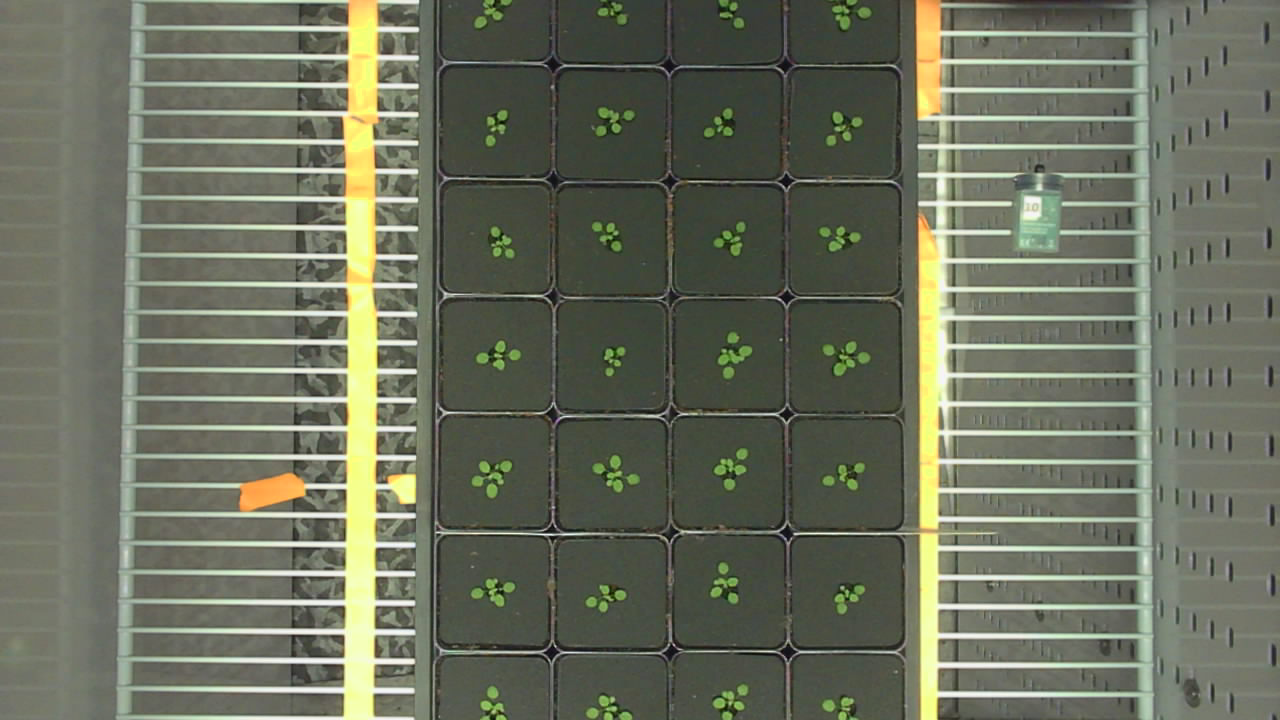
\includegraphics[width=.47\textwidth]{Figures/rawImages/a.png}\\
%Arabidopsis \\
%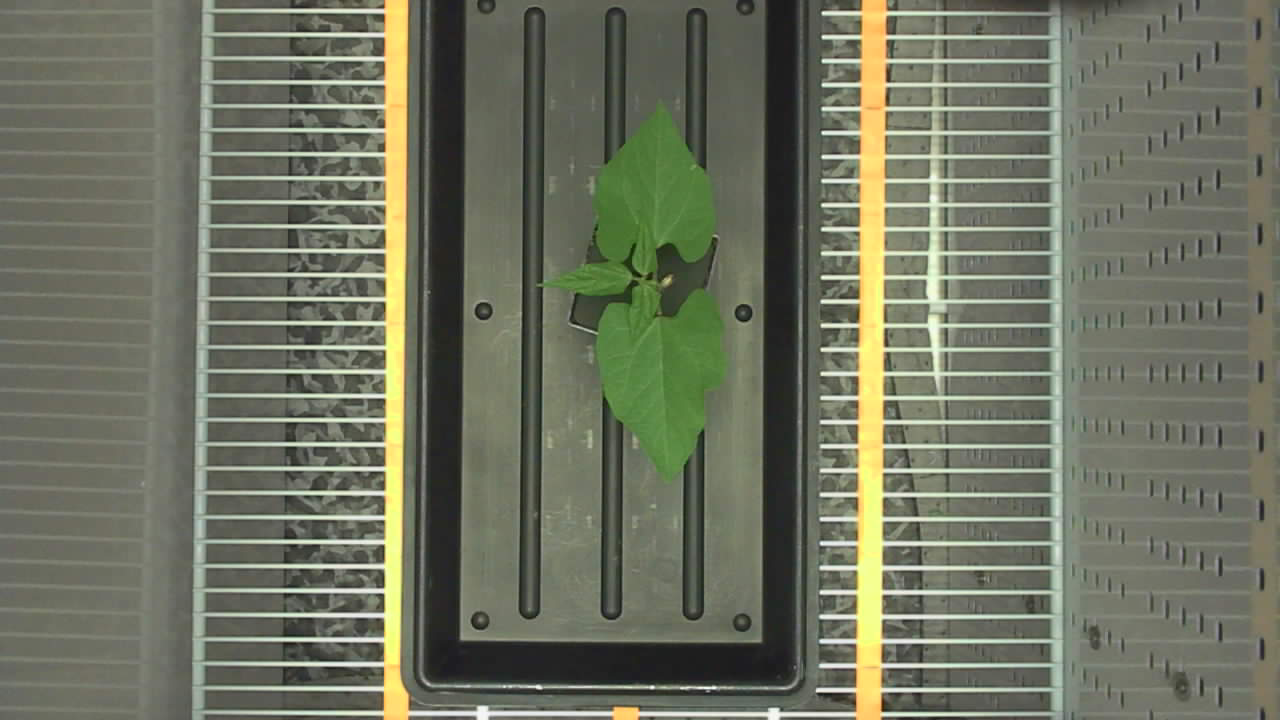
\includegraphics[width=.47\textwidth]{Figures/rawImages/b.png}\\
% Bean \\
%\end{tabular}
%\caption{RGB color images of Arabidopsis and bean plants. }
%\label{fig:rawIm}
%\end{centering}
%\end{figure}







\section{Annotation, Files and Protocol}
\subsection{Data Statistics}
MSU-PID includes two subsets, one for each plant type: Arabidopsis and bean.
The statistic information of these two subsets are summarized in Table~\ref{tab:stat}.
The images were acquired every hour.
As there is no light at night hours, plants can not be imaged by the fluorescence and RGB color sensors while IR and depth cameras can still perform the capturing during the night.
In order to make sure that all four modalities are present at the same time, we release the part of images captured only in the day hours, which are $15$ images per day for Arabidopsis and $13$ for bean for all four modalities.

The two subsets differ in image resolutions.
As shown in Figure~\ref{fig:fourmodality}, we grow and image a single bean plant while a whole tray of Arabidopsis are grown at the same time.
Therefore, the resolution of a Arabidopsis image is much lower than that of a bean image.
We manually crop $16$ Arabidopsis plants, which have been captured by all three cameras simultaneously.
Table~\ref{tab:resolution} summaries the image resolution of each plant in all four modalities.


\begin{figure*}
\centering
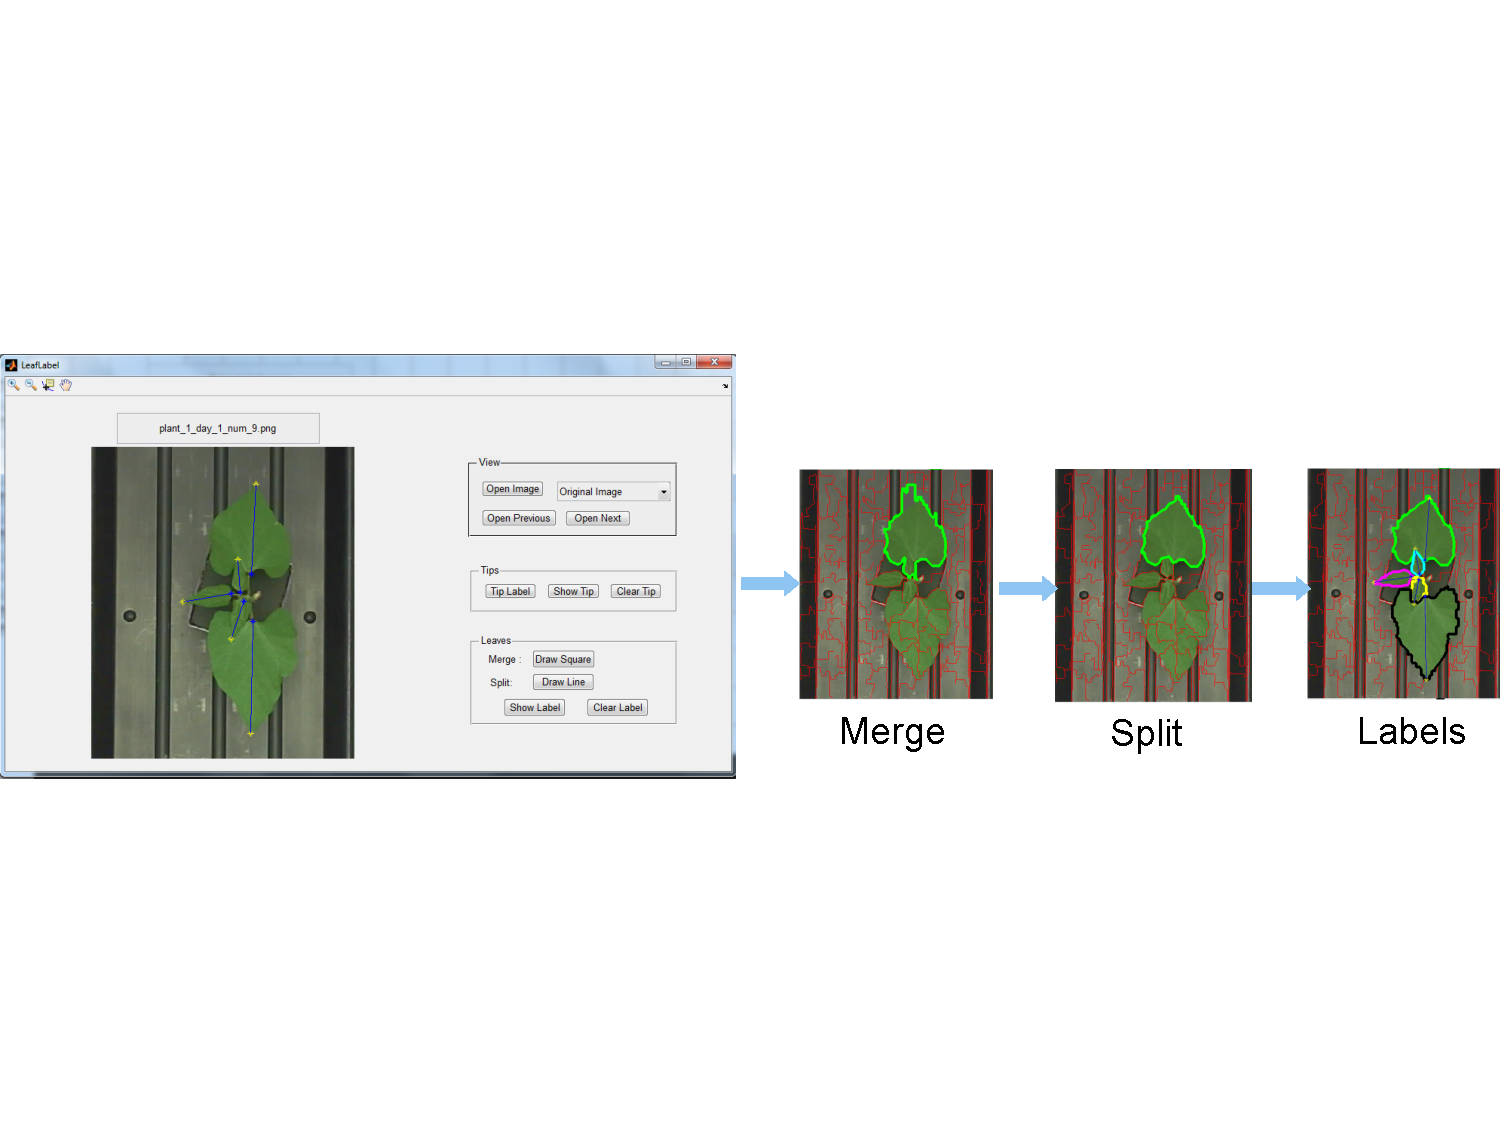
\includegraphics[width=.90\textwidth]{Figures/labeling}\\
\caption{Leaf annotation process, including leaf tip and leaf segment labels.}
\label{fig:label}
\end{figure*}

%\begin{figure*}
%\begin{centering}
%\begin{tabular}{@{}c@{} c@{} c@{} c@{} c@{} c@{} c@{} c@{} c@{}}
%%\begin{tabular}{lllllllll}
%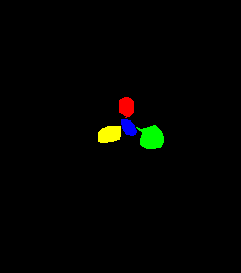
\includegraphics[width=.11\textwidth]{Figures/labelExample/plant_1_day_1_num_13.png}&
%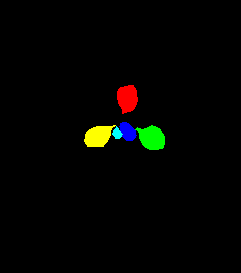
\includegraphics[width=.11\textwidth]{Figures/labelExample/plant_1_day_2_num_13.png}&
%
\includegraphics[width=.11\textwidth]{Figures/labelExample/plant_1_day_3_num_13.png}&
%
\includegraphics[width=.11\textwidth]{Figures/labelExample/plant_1_day_4_num_13.png}&
%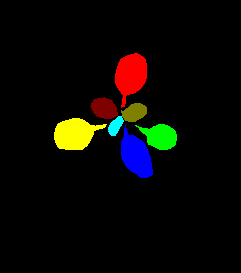
\includegraphics[width=.11\textwidth]{Figures/labelExample/plant_1_day_5_num_13.png}&
%
\includegraphics[width=.11\textwidth]{Figures/labelExample/plant_1_day_6_num_13.png}&
%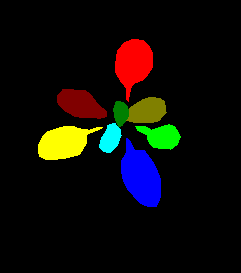
\includegraphics[width=.11\textwidth]{Figures/labelExample/plant_1_day_7_num_13.png}&
%
\includegraphics[width=.11\textwidth]{Figures/labelExample/plant_1_day_8_num_13.png}&
%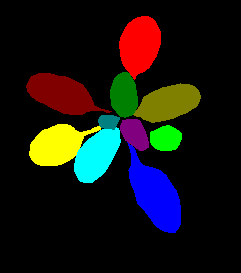
\includegraphics[width=.11\textwidth]{Figures/labelExample/plant_1_day_9_num_13.png}\\
%day 1 & day 2 & day 3 & day 4 & day 5 & day 6 & day 7 & day 8 & day 9 \\
%\end{tabular}
%\caption{Leaf labeling results of one Arabidopsis plant over nine days with one image per day. Note that the labels of tips are not shown for visualization clarity. }
%\label{fig:LabelExample}
%\end{centering}
%\end{figure*}

%It is often argued which is the best setting due to the trade-off between the image resolution and the throughput of phenotyping experiments.
The trade-off between image resolution and sample throughput is a common conundrum with designing visual phenotyping experiments.
We chose to image a whole tray of Arabidopsis at lower resolution rather than an individual at higher resolution, because it better reflects high-throughput protocols, which in practice allow direct comparison of multiple genotypes in the same experiment.
In contrast, we chose to image a single bean plant because we anticipate enabling development of $3$D plant canopy reconstruction algorithms for bushy plants.


\subsection{Manual Annotations}
\label{sec:annotation}
Part of the database is manually annotated to provide ground truth tip locations, leaf segmentation results, and leaf consistency overtime.
We use the fluorescence images as the input for labeling because of their clean and uniform background.
%Tip locations are saved in a TXT file for each frame.
%Leaf segmentation results are stored in a PNG image for each frame with one color for each leaf.
%The same color is used to represent the same leaf over a sequence of frames.

For Arabidopsis images, we labeled $4$ frames per day.
While for bean images, we labeled $7$ frames per day due to the plant's fast and spontaneous leaf movements.
A Matlab GUI interface was developed for leaf labeling, as shown in Figure~\ref{fig:label}, which will be released to the public.
A user can open a plant image (``Open") to label the two tips and annotate each leaf segment.
The results will be automatically saved once a user moves to a previous or next image (``Previous", and ``Next").
For consistent annotation of the same leaf over time, we show a number on the center of each leaf indicating the order of labeling from the previous frame.
The users should follow the order to label leaves. 

The labeling of the leaf segment (``Leaf Label") is implemented by clicking the boundary of one leaf at each time.
In order to provide more accurate labeling, a fairly high point density ($\sim20$ points on average) is typically used to define the boundary for each leaf. .
The labeled leaf boundary is overlaid on the image for better visualization to guide the next action.
An incorrect label can be deleted right after the labeling by clicking ``Clear", or all leaf labels can be deleted by clicking ``Clear All".
This process continues until all leaf segments have been annotated.
Once a leaf is invisible due to occlusion, the label can be skipped by clicking ``Invisible".

The labeling of leaf tips (``Tip Label") is implemented by clicking pairs of points on the image.
The outer tip is always clicked first before the inner tip.
For visualization, a line connecting each pair of tips will be shown immediately after clicking the inner tip.
Inaccurate labels can be deleted by clicking the right button of the mouse near the labeled point and relabeled by clicking the left button again immediately after deletion.
All tips can be deleted by clicking ``Clear Tip" and relabel again.
The ``Show Tip" option is to select whether to show the tips or not.
For relabeling of both leaf segments and leaf tips on the current image, click ``Restart".

After the labeling, we visually go through the results and correct inaccurate labels.
One example of the labeling results for one plant is shown in Figure~\ref{fig:trackExample} $(b)$, where one color is used to represent each specific leaf.
As we can see during the transition between day $5$ and day $6$, there is one leaf showing up and covering up the leaf underneath, which disappears and will not be annotated later.
% In total, we labeled $5,142$ leaves for fluorescence images.

Note that one alternative approach for labeling leaf segments is to directly label the membership of superpixels instead of drawing a polygon along the boundary.
Our experience is that since a noticeable percentage of extracted superpixels cover pixels of two neighboring leaves, the extra effort of breaking a super pixel into two makes it a less efficient alternative.


\subsection{Multimodal Annotations}
\begin{figure*}[t]
\begin{centering}
\begin{tabular}{cccc}
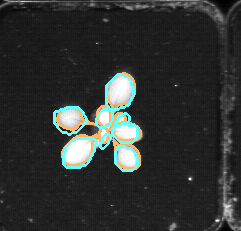
\includegraphics[width=.15\textwidth]{Figures/LabelAlignment/day_3_hour_23-seg_ir.png}&
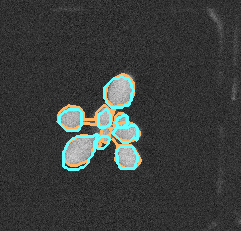
\includegraphics[width=.15\textwidth]{Figures/LabelAlignment/day_3_hour_23-seg_fmp.png}&
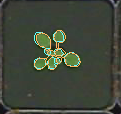
\includegraphics[width=.15\textwidth]{Figures/LabelAlignment/day_3_hour_23-seg_rgb.png}&
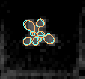
\includegraphics[width=.15\textwidth]{Figures/LabelAlignment/day_3_hour_23-seg_depth.png}\\
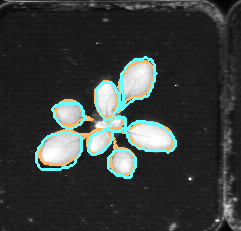
\includegraphics[width=.15\textwidth]{Figures/LabelAlignment/day_5_hour_23-seg_ir.png}&
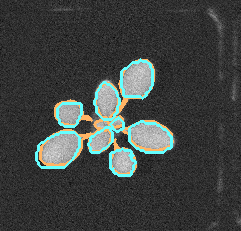
\includegraphics[width=.15\textwidth]{Figures/LabelAlignment/day_5_hour_23-seg_fmp.png}&
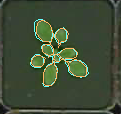
\includegraphics[width=.15\textwidth]{Figures/LabelAlignment/day_5_hour_23-seg_rgb.png}&
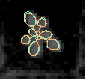
\includegraphics[width=.15\textwidth]{Figures/LabelAlignment/day_5_hour_23-seg_depth.png}\\
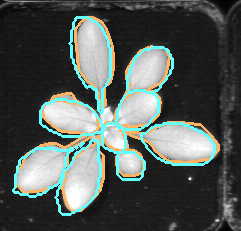
\includegraphics[width=.15\textwidth]{Figures/LabelAlignment/day_9_hour_20-seg_ir.png}&
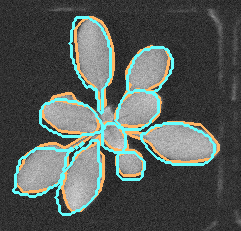
\includegraphics[width=.15\textwidth]{Figures/LabelAlignment/day_9_hour_20-seg_fmp.png}&
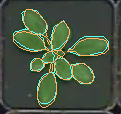
\includegraphics[width=.15\textwidth]{Figures/LabelAlignment/day_9_hour_20-seg_rgb.png}&
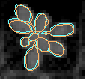
\includegraphics[width=.15\textwidth]{Figures/LabelAlignment/day_9_hour_20-seg_depth.png}\\
($a$) & ($b$) & ($c$) & ($d$) \\
\end{tabular}
\caption{Label propagation between all four modalities ($a$) IR, ($b$) fluorescence, ($c$) RGB color, and ($d$) depth, of a sample plant in the Arabidopsis collection for day $3$ (top row), day $5$ (middle row), and day $9$ (bottom row).
In the dataset the manual segmentation is performed on the fluorescence images and is outlined here as orange lines propagated to all modalities (i.e., the orange lines in (b) are manual labels while these in other three modalities are propagated labels).
The IR images are taken by the same camera and so will have exact pixel correspondence.
To assess the segmented pixel propagation to other modalities, we also manually labeled a subset of the color plant images (shown as cyan in (c)) and propagated this label to other three modalities (i.e., the cyan in (a,b,d) are propagated labels).
Comparing these boundaries in each modality gives a measure of the propagation errors due to parallax, and we provide quantitative analysis in Table~\ref{tab:labelError}.
Note that the color and depth images are rotated $90$ degrees.}
\label{fig:LabelAlignment}
\end{centering}
\end{figure*}

The leaf labeling can be propagated from the fluorescence images to each of the other modalities for the Arabidopsis sequences.
To do this, we approximate a plant image with a plane, and estimate homographies that transform the fluorescence images into the images in other modalities.
This provides a direct mapping of the pixel labels between each modality.
% and is illustrated in Figure~\ref{fig:LabelAlignment}.

To quantify the precision of the label propagation, we manually label $3$ images for each of $3$ Arabidopsis plants ($9$ images in total) on fluorescence and RGB modalities.
The labels in each modality is propagated on other modalities.
The result of one plant is illustrated in Figure~\ref{fig:LabelAlignment}.
This mapping will introduce errors due to depth-based parallax.
We use {\it{SBD}} score, which will be introduced in Section~\ref{sec:protocol}, to evaluate the similarity between the manual labels and the propagated labels.
In order to compute the inter-annotators variability, we ask two different annotators to label the same $9$ images and compute the {\it{SBD}} score.
The results are shown in Table~\ref{tab:labelError}.

We can make two conclusions from Table~\ref{tab:labelError}.
First, the similarity for both manual annotation and label propagation increases as the plant grows.
This is expected because {\it{SBD}} depends on the overlap ratio between two leaves, which inherently favors large leaves.
Second, the performance of label propagation is only slightly worse than the performance of human annotations.
Therefore, we use label propagation to provide the labels for all four modalities for Arabidopsis sequences.
There are two benefits: $1)$ it decreases the need for manual label; $2)$ labeling is consistent for all four modalities.
%, which not only saves laborious human labor, but also provides consistent labels for all four modalities.

\begin{table}[h]
\centering
\caption{Human label performance vs. label propagation performance.
$L_1$ and $L_2$ are the manual label results from two annotators, and $L_t$ is the propagated results.
The {\it{SBD}} score is averaged over $3$ plants.}
\begin{tabular}{c|c|c|c|c}
\hline
    & \multicolumn{2}{c|}{fluorescence} & \multicolumn{2}{c}{RGB}\\ \hline
    & $L_1$ vs. $L_2$  & $L_1$ vs. $L_t$ & $L_1$ vs. $L_2$ & $L_1$ vs. $L_t$ \\ \hline
   day$\_3$ & $0.808$ & $0.804$ & $0.827$ & $0.802$ \\ \hline
   day$\_5$ & $0.830$ & $0.836$ & $0.871$ & $0.837$ \\ \hline
   day$\_9$ & $0.903$ & $0.886$ & $0.877$ & $0.789$ \\ \hline
    average &   $0.847$ & $0.842$ & $0.858$ & $0.809$ \\ \hline
\end{tabular}
\label{tab:labelError}
\end{table}


In the case of the bean sequences, the pixel association between modalities is more difficult as the within-plant depth variations are large.
We found that a homograph-based mapping performed poorly, and so the manual annotations we supply apply to just the infrared and fluorescence images that use the same camera.


\subsection{Name Conventions and File Types}
We release training and testing sets in two separate folders.
In each folder, there are two subfolders named Arabidopsis and Bean.
The files in each subfolder have the following form:

\begin{itemize}
%\item plant$\_$ID$\_$day$\_$X$\_$hour$\_$YY$\_$rgb.png: the original RGB color images;
%\item plant$\_$ID$\_$day$\_$X$\_$hour$\_$YY$\_$fmp.png: the original fluorescence images;
%\item plant$\_$ID$\_$day$\_$X$\_$hour$\_$YY$\_$ir.png: the original IR images;
%\item plant$\_$ID$\_$day$\_$X$\_$hour$\_$YY$\_$depth.png: the original depth images;
\item plant$\_$ID$\_$day$\_$X$\_$hour$\_$YY$\_$modality.png: the original images in each modality separately;
%\item plant$\_$ID$\_$day$\_$X$\_$hour$\_$YY$\_$label.png: the labeled images of fluorescence modality;
%\item plant$\_$ID$\_$day$\_$X$\_$hour$\_$YY$\_$tips.txt: the labeled tip locations;
\item plant$\_$ID$\_$day$\_$X$\_$hour$\_$YY$\_$label$\_$modality.png: the labeled images of each modality if available;
\item plant$\_$ID$\_$day$\_$X$\_$hour$\_$YY$\_$tips$\_$modality.txt: the labeled tip locations of each modality if available;
\item plant$\_$ID$\_$day$\_$X$\_$hour$\_$YY$\_$depthSigma.png: the depth standard deviation images;
\end{itemize}
where ID indicates the plant subject ID number ($1$ to $16$ for Arabidopsis, $1$ to $5$ for bean), X is an integer indicating the date ($1-9$ for Arabidopsis, $1$ to $5$ for bean), and YY represents the hour index within a day ($9-23$ for Arabidopsis, $9-21$ for bean).
For each combination of day and hour, we provide the original images in all four modalities ($\_$rgb, $\_$fmp, $\_$ir, $\_$depth) in PNG files.
%\begin{itemize}
% \item plant$\_$XX$\_$day$\_$X$\_$hour$\_$YY$\_$ID$\_$ZZ$\_$rgb.png: the original RGB color images;
% \item plant$\_$XX$\_$day$\_$X$\_$hour$\_$YY$\_$ID$\_$ZZ$\_$fmp.png: the original fluorescence images;
% \item plant$\_$XX$\_$day$\_$X$\_$hour$\_$YY$\_$ID$\_$ZZ$\_$ir.png: the original IR images;
% \item plant$\_$XX$\_$day$\_$X$\_$hour$\_$YY$\_$ID$\_$ZZ$\_$depth.png: the original depth images;
% \item plant$\_$XX$\_$day$\_$X$\_$hour$\_$YY$\_$ID$\_$ZZ$\_$label.png: the labeled images of fluorescence modality;
% \item plant$\_$XX$\_$day$\_$X$\_$hour$\_$YY$\_$ID$\_$ZZ$\_$tips.txt: the labeled tip locations;
%\end{itemize}
%where XX indicates the plant type ("AR" or "BE"), X is an integer indicating the date (e.g., $1-9$ for Arabidopsis), YY represents the image index within a day (e.g., $1-16$ for Arabidopsis), and ZZ is the subject (or plant) ID (e.g., $1-5$ for bean).
%For each combination of day and hour, we provide four modalities in PNG files ($\_$rgb, $\_$fmp, $\_$ir, $\_$depth).
For annotated modalities, we have two additional files ($\_$label, $\_$tips) saving the annotation results.
Leaf segmentation results are encoded as indexed PNG files, where each leaf is assigned a unique and consistent leaf ID over time.
Leaf ID starts from $1$ and continuously increases till the total number of leaves.
And the background is encoded as $0$.
Tips locations are saved in TXT files where each line has the following format:
\begin{itemize}
\item leaf ID \quad tip1$\_$x \quad tip1$\_$y \quad tip2$\_$x \quad tip2$\_$y
\end{itemize}
where leaf ID is an integer number that is consistent with the segmentation label in the $\_$label file.
tip$1\_$x and tip$1\_$y represent the coordinates of the outer tip point.
tip$2\_$x and tip$2\_$y represent the coordinates of the inner tip point.
Any ``nan" value in the file indicates an invisible leaf.


%In addition to the original images and annotation results, we provide another folder named Matlab with all Matlab functions that will be used for mapping between different image modalities and for the purpose of performance evaluation.
%Note that the annotation is provided based on fluorescence images.
%In order to evaluate methods developed on other modalities, we provide image-mapping functions between every two modalities.
The total storage of our database is around $380 MB$, which is convenient for downloading via Internet.

\begin{figure*}[t!]
\centering
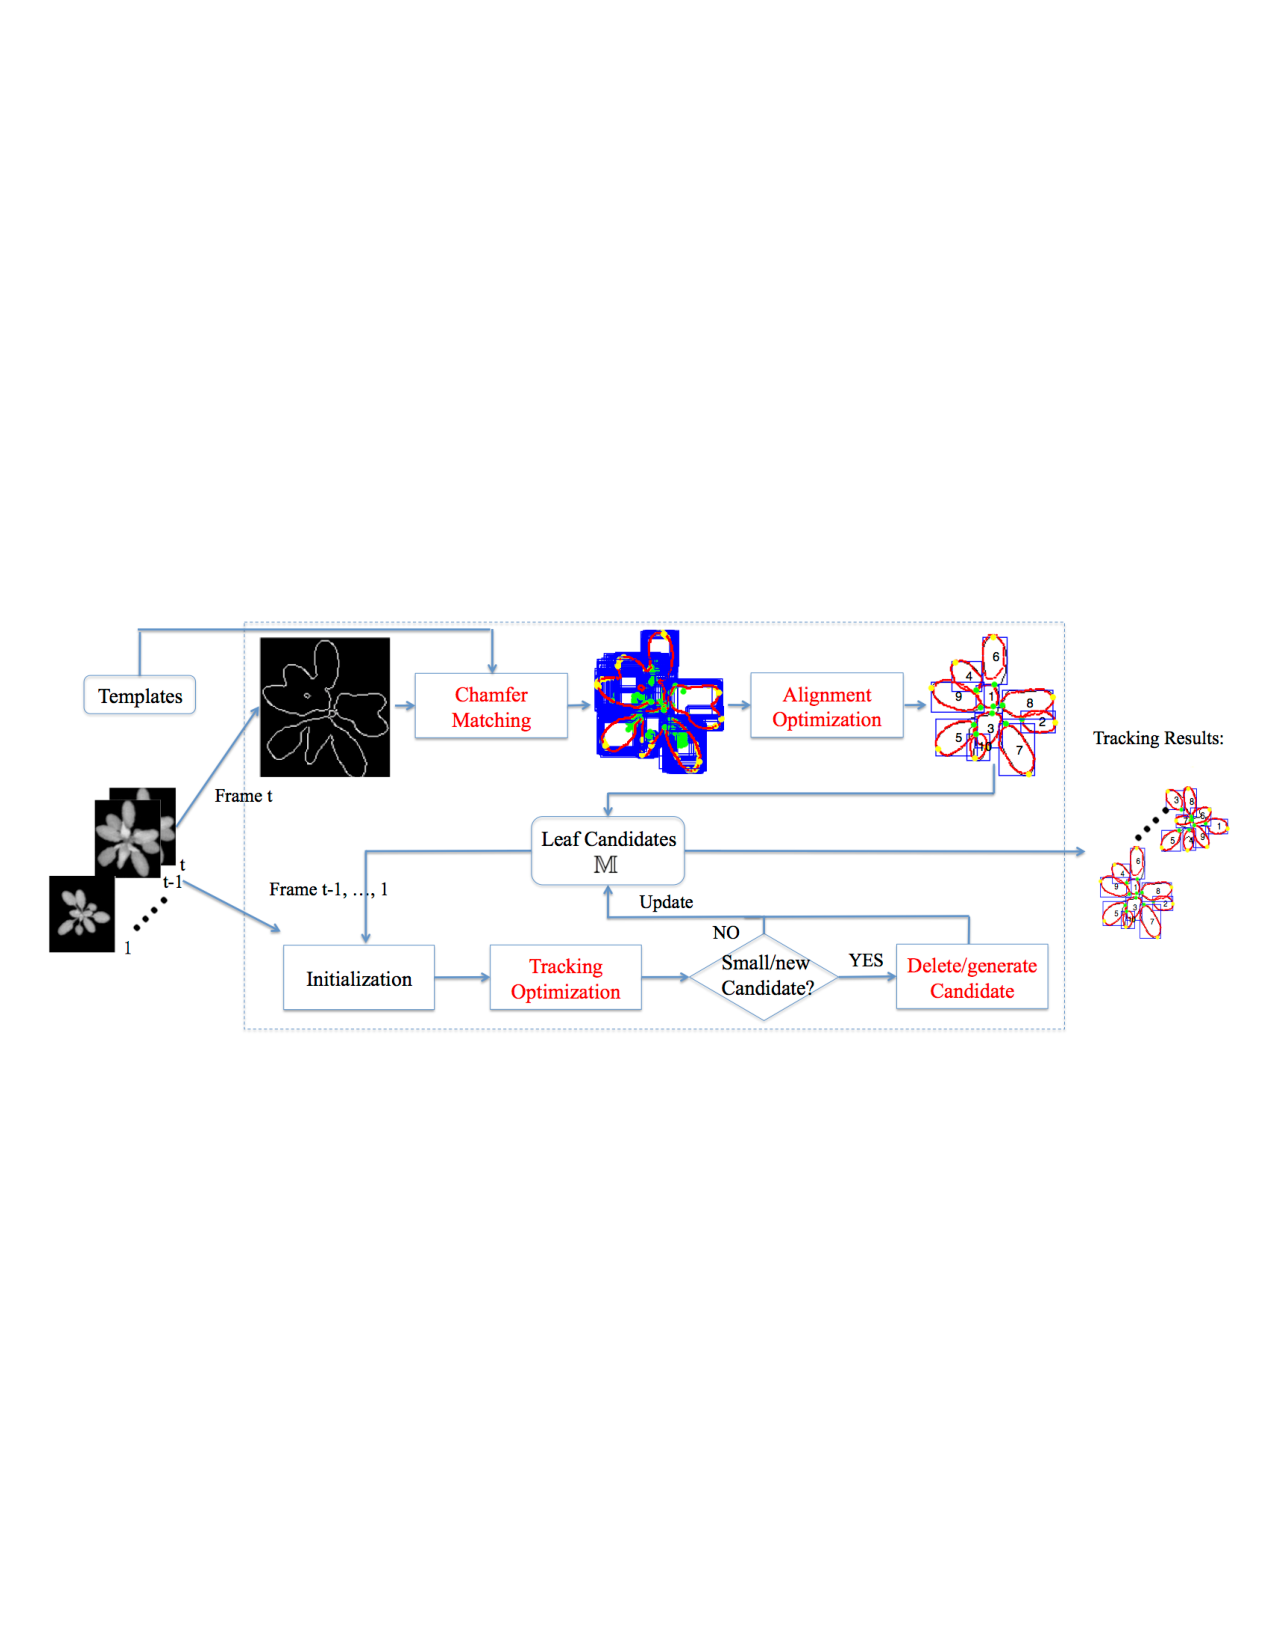
\includegraphics[width=.98\textwidth]{Figures/overview}\\
\caption{Overview of the baseline method.}
\label{fig:methodOverview}
\end{figure*}

\subsection{Experimental Protocols}
\label{sec:protocol}
As shown in Table~\ref{tab:database}, MSU-PID can be used for applications such as leaf segmentation, leaf counting, leaf alignment, and leaf tracking.
To facilitate future research, we separate the database into training set and testing set.
$40\%$ of the data is used for training and $60\%$ for testing.
Specifically, $6$ plants of Arabidopsis and $2$ plants of bean are selected for training.
%We will provide training and testing data in different folders.
For fair comparison, both supervised learning and unsupervised learning methods should evaluate their performance on the training and testing sets separately.

The user may decide to utilize one or multiple modalities of the plant imagery for training and testing respectively.
The availability of multiple modalities allows user to design novel experimental setup.
For example, using RGB and depth modalities for training and RGB for testing can take advantage of additional information during the learning without incurring extra sensor cost during the testing, which can be implemented via either learning with side information~\cite{chen2013boosting}, or transfering learning with missing modality~\cite{ding2014latent}.


\paragraph{Performance Metric}
To evaluate the performance of leaf segmentation, alignment, tracking, and counting, we use four performance metrics, whose Matlab implementations will be provided along with the data.
Three of them are based on the tip-based error, which is defined as the average distance of a pair of estimated leaf tips $\hat{\bm{t}}_{1,2}$ with a pair of labeled leaf tips $ \bm{t}_{1,2}$ normalized by the labeled leaf length:
\begin {equation}
e_{la}(\hat{\bm{t}}_{1,2}, \bm{t}_{1,2}) = \frac{||\hat{\bm{t}}_1-{\bm{t}}_1||_2 + ||\hat{\bm{t}}_2-{\bm{t}}_2||_2}{2 ||\bm{t}_1-\bm{t}_2||_2}.
\label{eqn:tipError}
\end{equation}

We build the frame-to-frame and video-to-video correspondence respectively and generate two sets of tip-based errors.
More details can be find in~\cite{yin2015}.
We define a threshold $\tau$ to operate on the corresponding tip-based errors.
By varying $\tau$, we compute the first three metrics as follows:
\begin{itemize}
\item {\it{Unmatched Leaf Rate (ULR)}}, the percentage of unmatched leaves with respect to the total number of labeled leaves.
This can attribute to two sources.
The first is miss detections and false alarms.
The second is matched leaves with tip-based errors larger than $\tau$.
When $\tau$ is large enough, this value is equal to the leaf counting error.
\item {\it{Landmark Error (LE)}}, the average tip-based errors smaller than $\tau$ of all frame-to-frame correspondent leaves.
This is used to measure the leaf tip alignment error.
\item {\it{Tracking Consistency (TC)}}, the percentage of video-to-video correspondent leaves whose tip-based errors are smaller than $\tau$.
This is used to measure leaf tracking accuracy.
\end{itemize}

In order to evaluate the leaf segmentation accuracy, we adopt an additional metric~\cite{scharr2014annotated} based on the Dice score of estimated segmentation results and ground truth labels:
\begin{itemize}
\item {\it{Symmetric Best Dice (SBD)}}, the average symmetric best Dice among all labeled leaves.
\end{itemize}
The Matlab function for computing {\it{SBD}} is provided by~\cite{scharr2014annotated}.
%The instructions on how to use the evaluation functions are included as comments of the function.


%For leaf annotation, we use the idea of merging and splitting super pixels.
%There are six different numbers of super pixels: $100$, $200$, $300$, $500$, $800$, $1000$.
%The user can specify which level to use depending on how well the super pixels can separate the leaves from the background.
%Because one leaf can be covered by several super pixels and one super pixel can across two leaves or the foreground and background.
%We allow merging and splitting super pixels.
%Merging is implemented by drawing a rectangle on the image.
%Every super pixel overlapping with this rectangle will be merged together.
%Splitting is implemented by drawing a line separating a leaf from the background or from another leaf.
%
%As shown in Figure ~\ref{fig:label}, several super pixels that covers one leaf are first merged together to form a large super pixel.
%Since the top part of the super pixel covers some of the background and the bottom part covers another small leaf, two lines are drawn on this super pixel to split it.
%The leaf boundary is overlaid on the image for better visualization to guide the next action.
%This process continues until all leaves have been annotated.


\section{Baseline Method and Performance}
\label{sec:baseline}

To facilitate future research on this database, we provide a baseline approach and its performance by using the fluorescence modality. 

\subsection{Multi-leaf segmentation and tracking framework}
We apply our automatic multi-leaf segmentation and tracking framework~\cite{yin2014a,yin2014b} to the testing set of Arabidopsis fluorescence imagery to provide a baseline.
As shown in Figure~\ref{fig:methodOverview}, the input of this framework is a plant video and a set of predefined templates with various shapes, scales, and orientations.
To generate the template set, we first select $10$ templates with different aspect ratios from the labeled images in the training set together with the corresponding tip locations.
For each template, we scale it to $12$ different sizes in order to cover the entire range of leaf sizes in the database.
For each scale template, we rotate every $15^{\circ}$ to generate $24$ templates at different orientations.
Tip locations will be scaled and rotated accordingly.
Finally, we generate $2,880$ leaf templates.

\begin{figure*}
\centering
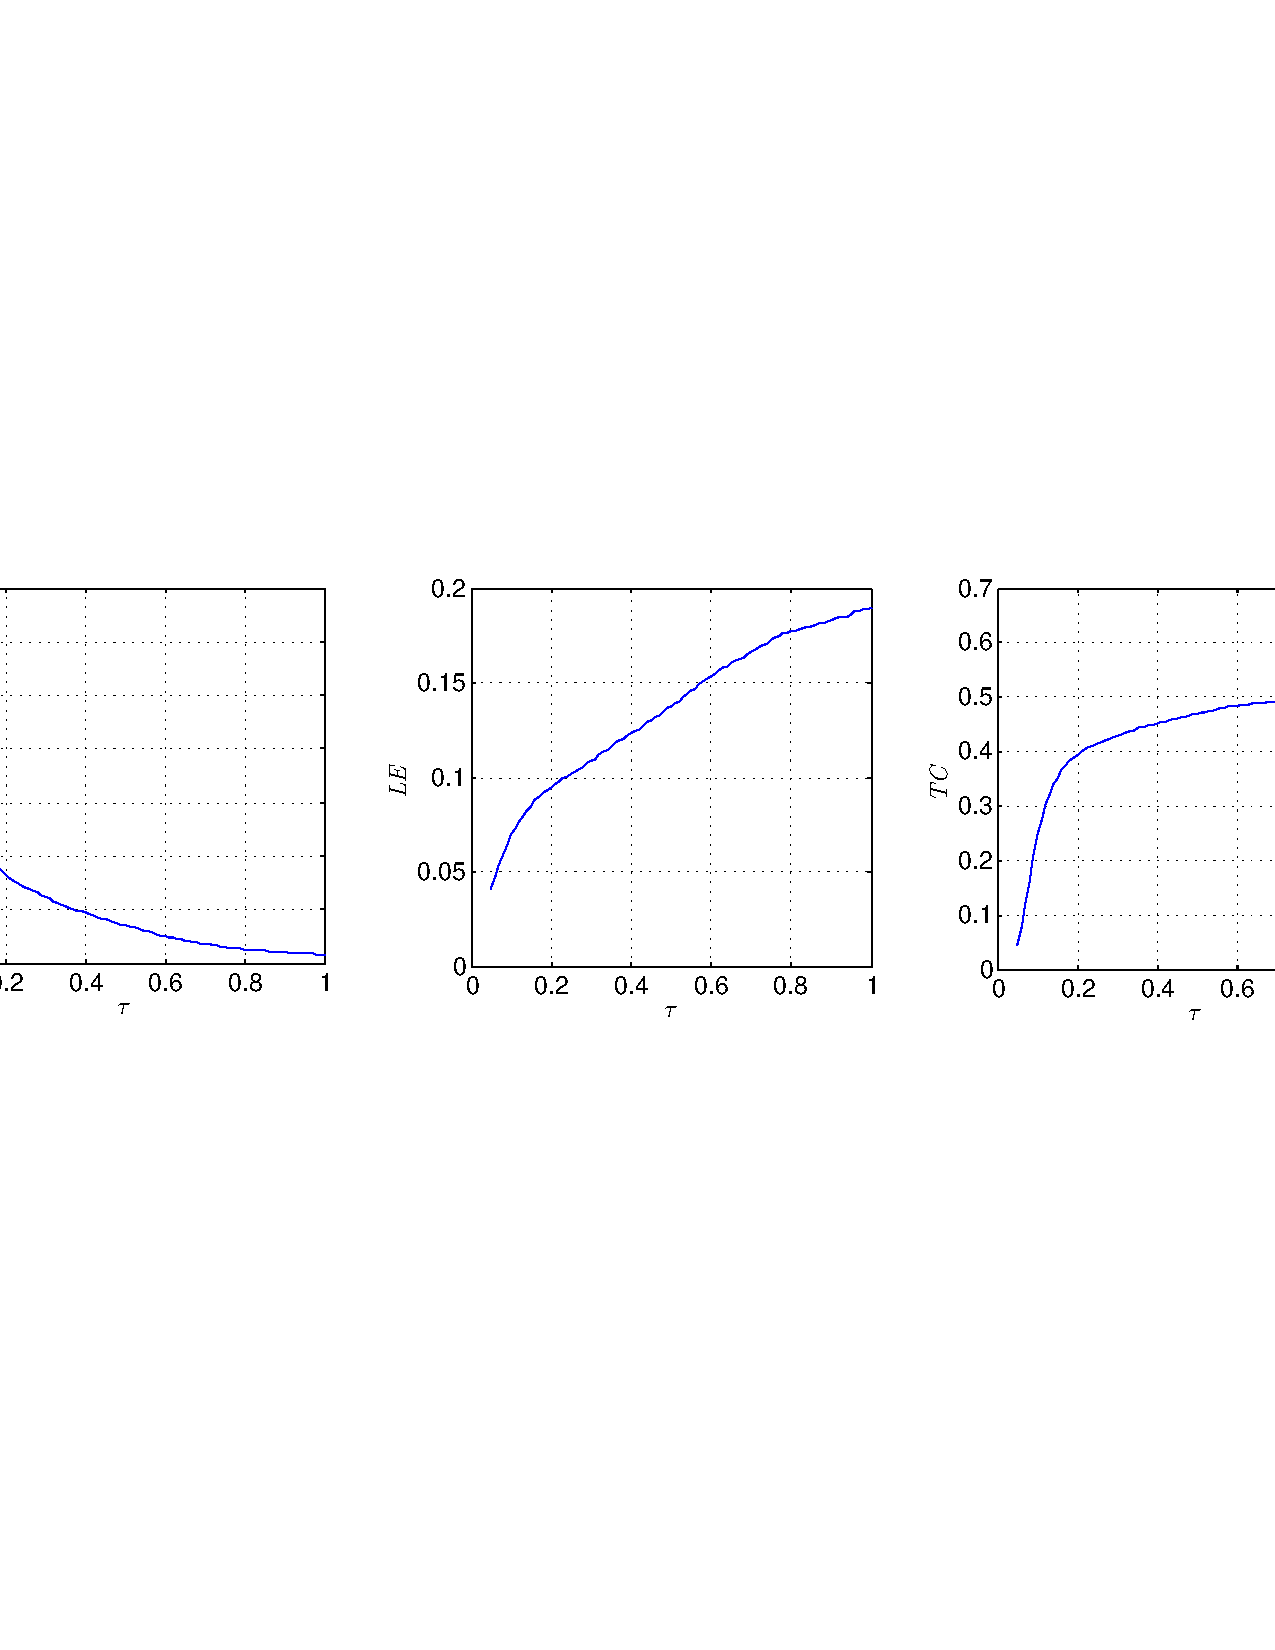
\includegraphics[width=.98\textwidth]{Figures/performance}\\
\caption{Performance of the baseline method.}
\label{fig:performance}
\end{figure*}

%We also generate the two tips for each template for finding the corresponding tip points of each leaf via Chamfer Matching~\cite{barrow1977parametric}.
Our work is motivated by Chamfer Matching technique~\cite{barrow1977parametric}, which is used to align two edge maps.
We extend it to simultaneously align multiple overlapping objects.
For each image, we use simple thresholding and edge detection to generate an edge map and mask.
First, we find the best location of each template in the edge map that has the minimal Chamfer matching distance, which will result in an over-completed set of leaf candidates.
Second, we apply multi-leaf alignment~\cite{yin2014a} approach to find an optimal set of leaf candidates on the last frame of the video, which will provide the information of the number of leaves, tip locations and boundaries of each leaf.
Third, we apply multi-leaf tracking~\cite{yin2014b} approach, which is based on leaf template transformation, to track leaves between continuous two frames.

In the tracking process, we develop a procedure to generate new leaves and delete small leaves.
For each frame of the video, we can generate a label image with each leaf being labeled with one color and the tip locations for each estimated leaf.
The labeled color for each leaf in the video remains the same during the tracking process.


\subsection{Performance and analysis}
The results of our algorithm by varying $\tau$ from 0 to 1 is shown in Fig.~.
And the {\it{SBD}} score is $0.51$ by averaging over all plants.







\section{Conclusion and Discussion}

This paper presents a newly collected multi-modality plant imagery dataset ``MSU-PID''.
It has two subsets for Arabidopsis and bean plants respectively. 
Compared to existing databases in the field, MSU-PID uses multiple calibrated modalities including fluorescence, infrared, RGB color, and depth. 
Detailed image capture process and camera calibration are studied. 
We provide our manual labels about leaf tip locations, leaf segments, and leaf consistency over time on fluorescence modality. 
The labels are propagated to other modalities using homograph mapping for Arabidopsis imagery. 
Our annotations enable a wide variety of plant image analysis applications. 

It might be noticed that all plants in MSU-PID belong to the same genotype and no treatments applied.
This is because we think a fundamental issue with visual phenotyping, i.e. accurate and automated identification and tracking of individual leaves over developmental time scales (weeks), which importance has being highlighted in Introduction, needs to be solved before expending our goal to define group differences.
The inherent challenge in this issue is that as leaves emerge and grow, they change in size, position and shape and they may overlap or be overlapped by other leaves.
We emphasize more in leaf identification and tracking rather than developing methods to define group differences.

For others to use our dataset, we have designed an experimental protocol with various evaluation metrics for different applications.  
To facilitate future research, we apply our automatic multi-leaf segmentation, alignment, and tracking algorithm on the fluorescence and RGB modalities of Arabidopsis imagery, where the labels for RGB modality is provided via label propagation. 
Our methods performs better on fluorescence images than RGB images. 
This is due to three reasons. 
First, the algorithm is originally developed for fluorescence images. 
Second, the resolution of RGB images are much lower than that of fluorescence images. 
Third, the groudtruth labels for RGB images are generated through the mapping of fluorescence labels, which will cause some error. 
We recognize our dataset as very challenging dataset. 

We believe this new database will be beneficial to the research community in terms of algorithm development, performance evaluation, and identifying new research problems in plant image analysis.
Furthermore, We are also open to suggestions and comments from the users of this database to further enhance our imaging setup and capturing protocol, so that we can develop new databases in the future.

%This paper presents a newly collected multi-modality plant imagery database, ``MSU-PID''.
%Compared to existing databases in the field, MSU-PID not only has multiple calibrated modalities, but also enables a wide variety of plant image analysis applications.
%Therefore, we believe this new database will be beneficial to the research community in terms of algorithm development, performance evaluation, and identifying new research problems in plant image analysis.
%Furthermore, we are also open to suggestions and comments from the users of this database to further enhance our imaging setup and capturing protocol, so that we can develop new databases in the future.
%
%It might be noticed that all plants (respectively for Arabidopsis and bean) in MSU-PID belong to the same genotype and no treatments applied.
%%This would entail that the proposed dataset cannot be used to investigate computer vision algorithms or imaging modalities in relation to group differences. Could the authors comment on this? This is true. We are not comparing group differences, based on morphology (for example).
%This is because we think a fundamental issue with visual phenotyping, i.e. accurate and automated identification and tracking of individual leaves over developmental time scales (weeks), which importance has being highlighted in Introduction, needs to be solved before expending our goal to define group differences. The inherent challenge in this issue is that as leaves emerge and grow, they change in size, position and shape and they may overlap or be overlapped by other leaves.
%%I think that new text we have added more clearly emphasizes leaf identification and tracking over time rather than developing methods/algorithms to define group differences.
%
%


%\paragraph{Paragraph headings} Use paragraph headings as needed.
%\begin{equation}
%a^2+b^2=c^2
%\end{equation}
%
%% For one-column wide figures use
%\begin{figure}
%% Use the relevant command to insert your figure file.
%% For example, with the graphicx package use
%  
\includegraphics{example.eps}
%% figure caption is below the figure
%\caption{Please write your figure caption here}
%\label{fig:1}       % Give a unique label
%\end{figure}
%%
%% For two-column wide figures use
%\begin{figure*}
%% Use the relevant command to insert your figure file.
%% For example, with the graphicx package use
%  
\includegraphics[width=0.75\textwidth]{example.eps}
%% figure caption is below the figure
%\caption{Please write your figure caption here}
%\label{fig:2}       % Give a unique label
%\end{figure*}
%%
%% For tables use
%\begin{table}
%% table caption is above the table
%\caption{Please write your table caption here}
%\label{tab:1}       % Give a unique label
%% For LaTeX tables use
%\begin{tabular}{lll}
%\hline\noalign{\smallskip}
%first & second & third  \\
%\noalign{\smallskip}\hline\noalign{\smallskip}
%number & number & number \\
%number & number & number \\
%\noalign{\smallskip}\hline
%\end{tabular}
%\end{table}


%\begin{acknowledgements}
%If you'd like to thank anyone, place your comments here
%and remove the percent signs.
%\end{acknowledgements}

% BibTeX users please use one of
%\bibliographystyle{spbasic}      % basic style, author-year citations
%\bibliographystyle{spmpsci}      % mathematics and physical sciences
%\bibliographystyle{spphys}       % APS-like style for physics
%\bibliography{}   % name your BibTeX data base



{%\small
\bibliographystyle{springer}
%\bibliography{/Sharefolder/Dropbox/Bibliographies/abbrev_brief,/Sharefolder/Dropbox/Bibliographies/xl-literature}
\bibliography{abbrev,xl-literature,science}
}
\end{document}
% end of file template.tex

